% Options for packages loaded elsewhere
\PassOptionsToPackage{unicode}{hyperref}
\PassOptionsToPackage{hyphens}{url}
%
\documentclass[
  11pt,
]{article}
\usepackage{lmodern}
\usepackage{amssymb,amsmath}
\usepackage{ifxetex,ifluatex}
\ifnum 0\ifxetex 1\fi\ifluatex 1\fi=0 % if pdftex
  \usepackage[T1]{fontenc}
  \usepackage[utf8]{inputenc}
  \usepackage{textcomp} % provide euro and other symbols
\else % if luatex or xetex
  \usepackage{unicode-math}
  \defaultfontfeatures{Scale=MatchLowercase}
  \defaultfontfeatures[\rmfamily]{Ligatures=TeX,Scale=1}
\fi
% Use upquote if available, for straight quotes in verbatim environments
\IfFileExists{upquote.sty}{\usepackage{upquote}}{}
\IfFileExists{microtype.sty}{% use microtype if available
  \usepackage[]{microtype}
  \UseMicrotypeSet[protrusion]{basicmath} % disable protrusion for tt fonts
}{}
\makeatletter
\@ifundefined{KOMAClassName}{% if non-KOMA class
  \IfFileExists{parskip.sty}{%
    \usepackage{parskip}
  }{% else
    \setlength{\parindent}{0pt}
    \setlength{\parskip}{6pt plus 2pt minus 1pt}}
}{% if KOMA class
  \KOMAoptions{parskip=half}}
\makeatother
\usepackage{xcolor}
\IfFileExists{xurl.sty}{\usepackage{xurl}}{} % add URL line breaks if available
\IfFileExists{bookmark.sty}{\usepackage{bookmark}}{\usepackage{hyperref}}
\hypersetup{
  pdfauthor={Aaron D. Lightner; Edward H. Hagen; Department of Anthropology, Washington State University},
  hidelinks,
  pdfcreator={LaTeX via pandoc}}
\urlstyle{same} % disable monospaced font for URLs
\usepackage[margin=1in]{geometry}
\usepackage{graphicx,grffile}
\makeatletter
\def\maxwidth{\ifdim\Gin@nat@width>\linewidth\linewidth\else\Gin@nat@width\fi}
\def\maxheight{\ifdim\Gin@nat@height>\textheight\textheight\else\Gin@nat@height\fi}
\makeatother
% Scale images if necessary, so that they will not overflow the page
% margins by default, and it is still possible to overwrite the defaults
% using explicit options in \includegraphics[width, height, ...]{}
\setkeys{Gin}{width=\maxwidth,height=\maxheight,keepaspectratio}
% Set default figure placement to htbp
\makeatletter
\def\fps@figure{htbp}
\makeatother
\setlength{\emergencystretch}{3em} % prevent overfull lines
\providecommand{\tightlist}{%
  \setlength{\itemsep}{0pt}\setlength{\parskip}{0pt}}
\setcounter{secnumdepth}{5}
\usepackage{fancyhdr}
\fancyhf{}
\renewcommand{\headrulewidth}{0pt}
\rhead{\thepage}
\pagestyle{fancy}
\usepackage{fontspec}
\newfontfamily{\defaultfont}{Palatino Linotype}
\newfontfamily{\blockfont}{DejaVu Sans}
\usepackage[BlockElements]{ucharclasses}
\setDefaultTransitions{\defaultfont}{}
\setTransitionsFor{BlockElements}{\blockfont}{}  
\usepackage{setspace}
\usepackage[utf8]{inputenc}
\usepackage{pdflscape}
\usepackage{booktabs}
\usepackage{sectsty}
\usepackage{booktabs}
\usepackage{longtable}
\usepackage{array}
\usepackage{multirow}
\usepackage{wrapfig}
\usepackage{float}
\usepackage{colortbl}
\usepackage{pdflscape}
\usepackage{tabu}
\usepackage{threeparttable}
\usepackage{threeparttablex}
\usepackage[normalem]{ulem}
\usepackage{makecell}
\usepackage{xcolor}

\title{\LARGE \textbf{Acculturation and market integration are associated with greater trust among Tanzanian Maasai pastoralists}}
\author{Aaron D. Lightner and Edward H. Hagen \\ Department of Anthropology \\ Washington State University}
\date{}

\begin{document}
\maketitle
\begin{abstract}
Acting on socially learned information involves risk, especially when
the consequences imply certain costs with uncertain benefits. Current
evolutionary theories argue that decision-makers evaluate and respond to
this information based on context cues, such as prestige (the
\emph{prestige bias model}; PBM), and/or incentives (the \emph{risk and
incentives model}; RIM). We tested the roles of each in explaining trust
using a preregistered vignette-based study involving advice about
livestock among Maasai pastoralists. In exploratory analyses, we also
investigated how the relevance of each might be influenced by recent
cultural and economic changes, such as market integration and shifting
cultural values. Our confirmatory analysis failed to support the PBM,
and partially supported the RIM. Exploratory analyses suggested that
regional acculturation varied strongly between northern vs.~southern
areas, divided by a small mountain. Consistent with the idea that trust
varies with socially transmitted values and regional differences in
market integration, people living near densely populated towns in the
southern region were more likely to trust socially learned information
about livestock. Higher trust among market-integrated participants might
reflect a coordination solution in a region where traditional
pastoralism is beset with novel conflicts of interest.

Word count: 6759
\end{abstract}

\pagenumbering{gobble}

\newpage

\pagenumbering{arabic}

\hypertarget{introduction}{%
\section{Introduction}\label{introduction}}

Individuals must often make critical decisions based on information
provided by others who might be untrustworthy, either because their
information is poor or they have incentives to deceive. As an example,
suppose that a herder suggests to another where he should move his
livestock during the dry season to find grass and water. In a semi-arid
ecology such as northern Tanzania, this advice implies an unavoidable
cost (moving the herd to another area) with a large but uncertain
benefit. How should the herder decide if this advice is trustworthy?
(Here, we define ``trust'' as ``reliance upon {[}socially learned{]}
information\ldots about uncertain environmental states and their
accompanying outcomes in a risky situation''; Schlenker, Helm, \&
Tedeschi (1973), p.~419; see also Yamagishi, Kikuchi, \& Kosugi (1999).)

Current theories of social learning focus on the source of information
and/or risks of acting on the information. Some theories emphasize
evolved learning biases, triggered by cues such as the prestige of the
information source (Henrich, 2017; Richerson \& Boyd, 2005), which we
refer to as the \emph{prestige bias model} (PBM). Other theories
emphasize flexible copying based on incentives, i.e., expected outcomes
of acting on the information and possible conflicts of interest with the
information source (Binmore, 2011; Mercier, 2020; Morin, 2015), which we
refer to as the \emph{risk and incentives model} (RIM). In a
preregistered study, we test the PBM and the RIM among Maasai
pastoralists. Evaluating socially learned information is further
complicated when individuals traverse varying cultural and economic
contexts: Individuals who might be trusted sources of information in one
context might be mistrusted in another. We investigate these effects in
a \emph{post hoc} exploratory analysis.

\hypertarget{prestige-bias-model-of-trust-pbm}{%
\subsection{Prestige bias model of trust
(PBM)}\label{prestige-bias-model-of-trust-pbm}}

In the simplest models of social learning, individuals simply learn from
a random individual in the population (Rogers, 1988). Social learning
can be enhanced, however, by preferentially copying more knowledgeable
individuals. One strategy would be to assess the knowledge of all group
members via personal experience over time, and then choose to copy the
most knowledgeable individual(s). But this would be time consuming and
error prone -- \emph{directly} observing performances can be noisy,
leading a learner to misperceive competence (e.g., see Boyd \&
Richerson, 1985, pp. 92--94, ch.~8). Alternatively, dual inheritance
theorists argue that evolved context biases can solve this problem by
exploiting simple and \emph{indirect} social cues, triggering simple
decision rules (Richerson \& Boyd, 2005). Prestige bias involves
preferentially copying individuals with \emph{prestige} gained by
``freely conferred deference'' (Boyd \& Richerson, 1985; J. Henrich \&
Gil-White, 2001). This is efficient because it simplifies a complex
learning task into a much simpler one. Relying on such a cue can reduce
noise by ``averag{[}ing{]} over many performances, which can help reduce
the error in the learner's assessment of who to learn from'' (Henrich \&
McElreath, 2007, p. 559; see also Hill \& Kintigh, 2009). Prestige bias
is also adaptive because this simplification can be trusted across
socioecological contexts and generational time (Henrich \& McElreath,
2003). Modeling studies demonstrate that prestige can signal locally
relevant skills and/or expertise (Plourde, 2008), and naive learners can
trust prestige signals to acquire locally adaptive knowledge
(``information goods'') quickly and accurately in a wide range of
conditions (Panchanathan, 2010). As J Henrich et al. (2001) explain
(p.~345, emphasis added):

\begin{quote}
A substantial amount of cross-cultural ethnography (e.g., Dove 1993;
Hammel 1964; Rogers 1995; Moore 1957) and laboratory psychology (for a
summary, see Gil-White and Henrich 1999) suggests that humans everywhere
possess a tendency to copy prestigious individuals, i.e., those who
receive the most displays of respect/deference from others. This
mechanism embodies two shortcut heuristics. First, by preferentially
copying a ``bundle'' of cultural traits from prestigious individuals
(prestige correlates with skill/knowledge and often wealth) copiers can
rapidly acquire a repertoire of fitness-enhancing or success-oriented
traits (i.e., better-than-average solutions to the problems of life).
Second, \emph{rather than gradually learning via individual experience
who the most successful, knowledgeable, or skillful individuals are,
copiers rely on honest ethological and sociolinguistic signals of
respect that other individuals display toward such high status
individuals}.
\end{quote}

Empirical support for the PBM is mixed (Jiménez \& Mesoudi, 2019). In
support, food taboos among pregnant and breastfeeding women in Fiji
largely improved their health outcomes, and some of these taboos were
transmitted by prestigious elderly women (J. Henrich \& Henrich, 2010;
cf.~Placek, Madhivanan, \& Hagen, 2017). Prestige was also a reliable
indicator of hunting skill among the Hadza (Stibbard-Hawkes,
Attenborough, \& Marlowe, 2018) and Tsimane (von Rueden, Gurven, \&
Kaplan, 2008), although for the latter, ethnobotanical knowledge did not
predict prestige (Reyes-Garcia et al., 2008). In experiments, children
and adults use prestige cues to improve their performance in a novel
task, especially when they are performing poorly (Atkisson, O'Brien, \&
Mesoudi, 2012; Chudek, Heller, Birch, \& Henrich, 2012). Experiments
have also found that when cues of success are available, participants
will favor those cues over prestige cues (Brand, Heap, Morgan, \&
Mesoudi, 2020). Surveys of the ethnographic literature on social
learning among hunter-gatherers and on leadership, however, found little
evidence of prestige biased learning (Garfield, Garfield, \& Hewlett,
2016; Garfield, Hubbard, \& Hagen, 2019).

Because the PBM relies on a narrow, restricted range of cues, a
cost-accuracy tradeoff leaves room for costly or ``irrational''
behaviors with specific, unavoidable, maladaptive side effects (e.g.,
see Richerson \& Boyd, 2005, pp. 119--124, 156 for discussion). In
weaker versions of the PBM prestige is conceptualized as one important
cue among many, whereas in stronger versions of the PBM prestige can
override other cues and decisions thus sharply diverge from individual
self-interests, including non-adaptive food taboos (Aunger, 1994; J.
Henrich \& Henrich, 2010), market bubbles (Bell, 2013), and suicide
epidemics (Henrich \& McElreath, 2007; Mesoudi, 2009). This ambiguity
among possible interpretations in the prestige bias literature is
discussed in Morin (2016).

\hypertarget{risk-and-incentives-model-of-trust-rim}{%
\subsection{Risk and incentives model of trust
(RIM)}\label{risk-and-incentives-model-of-trust-rim}}

People might also be ``epistemically vigilant'', or largely resistant to
social influence while conditionally trusting advice based on message
content, risk, incentives, and perceived conflicts of interests with the
sender (Mercier \& Sperber, 2017; Trouche, Johansson, Hall, \& Mercier,
2018; see also Binmore, 2011; Hess \& Hagen, 2006; Mercier, 2020; Morin,
2015). If the trustworthiness of socially learned information is
questionable, the RIM emphasizes that acting on it is a \emph{gamble}
between two options, possibly with equivalent expected values, with a
low-variance safe option (high probability of receiving a low payoff)
and a high-variance risky option (lower probability of a high payoff).
Individuals preferring the safe option are \emph{risk averse}, and those
preferring the risky option are \emph{risk seeking}.

Which of these option types is adaptive depends strongly on an
organism's current state: Foragers with a sufficient energy budget, for
example, should be risk averse, whereas foragers with a dangerously low
energy budget should be risk seeking (Stephens, 1981). The relationship
between resource scarcity and risk seeking, mediated by stress, is
supported in non-human animal experiments manipulating energy budgets
(Caraco et al., 1990; Kacelnik \& Bateson, 1996), as well as
observational studies in humans (see Winterhalder, 2007 for review). As
biologists and economists have observed, this apparent risk sensitivity
of decision-making might be explained as maximizing long-term growth
rates under multiplicative dynamics (Kacelnik \& Bateson, 1996; Peters,
2019; Peters \& Gell-Mann, 2016; Price \& Jones, 2020).

Theoretical distinctions between social vs.~individual learning
strategies could distract from the fundamental task in most real-world
decision-making: weighing the expected costs and benefits (Morin, 2015).
If acting on social influence is cheap and outcomes are trivial, then a
useful decision rule should not seek more expensive cues; but if the
stakes are high enough, then a high cost for accuracy might be worth
paying.

Experimental evidence has supported some key aspects of the RIM in
humans. People are more likely to take high-risk decisions under stress
and resource scarcity (Dalton, Nhung, \& Rüschenpöhler, 2019; Kirchler
et al., 2017; Putman, Antypa, Crysovergi, \& van der Does, 2009),
although some experiments show that poverty induces risk aversion (a
poverty trap; Yesuf \& Bluffstone (2009)). In social contexts,
participants' evaluations of argument persuasiveness are conditioned on
how relevant the consequences of its message would be for them (Petty \&
Wegener, 1998). If consequences are not relevant, then people rely on
social information and heuristics such as expertise and audience
approval (Axsom, Yates, \& Chaiken, 1987). If they are relevant, then
they evaluate the content of the message (Petty, Cacioppo, \& Goldman,
1981). Content evaluation might trend toward psychologically attractive
ideas (Miton, Claidière, \& Mercier, 2015), individual preferences
(Acerbi \& Tehrani, 2018), or attempts to reduce the ambiguity of social
cues when multiple cues are available (Conway \& Schaller, 2005). People
are sensitive to conflicts of interest and social informational
``dependencies'' (Hess \& Hagen, 2006; Mercier \& Miton, 2019), and are
more likely to trust expert advice when they are given clear
demonstrations of expertise rather than an argument from expertise
(Mercier et al., 2019).

\hypertarget{the-impact-of-changing-ideational-and-material-culture-on-trust}{%
\subsection{The impact of changing ideational and material culture on
trust}\label{the-impact-of-changing-ideational-and-material-culture-on-trust}}

Another perspective, which is consistent with the RIM and some
interpretations of the PBM, is that decisions about social information
can flexibly adapt to variation in ``ideational'' (values and norms) and
``material'' (economic) culture. If widespread incentives are suddenly
distorted by changing material conditions, such as market integration
and/or developing infrastructure, then ideational changes might
predictably follow (Aoki, 2011; Binmore, 2011; Yamagishi \& Suzuki,
2009). Proponents of this view often start from an assumption of
\emph{methodological individualism}, similar to the RIM (i.e., social
phenomena are grounded in individual incentives; see North (1990)).
Market integration in developing nations and small-scale societies
imposes novel transaction costs, which can in turn disrupt existing
sharing institutions and undermine widespread trust (e.g., Ensminger,
1992; Baird, 2014; Kasper \& Borgerhoff Mulder, 2015). This might render
social status, kinship, and reciprocity insufficient for establishing
trust in most social interactions. This would create a demand for
culturally evolved norms to sustain mutually beneficial exchanges, such
as fairness and/or religious beliefs that stabilize trust by
manipulating perceived incentives (J. Henrich et al., 2010) or encourage
use of inferred mental states in moral judgements (Curtin et al., 2020).
Costly religious rituals also signal trustworthiness among strangers
(Ensminger, 1997; Power, 2017), and religious beliefs in omniscient,
moralistic gods stabilize trust in large-scale, market-integrated
communities (Lang et al., 2019; Purzycki et al., 2016).

\hypertarget{study-aims-and-context}{%
\subsection{Study aims and context}\label{study-aims-and-context}}

Here, we (1) test the PBM and RIM as models of trust using a
vignette-based experiment involving advice about livestock among Maasai
pastoralists, and (2) conduct an observational study of the impact of
recent cultural and economic changes, such as market integration and
shifting cultural values, on trust.

\hypertarget{preregistered-predictions}{%
\subsubsection{Preregistered
predictions}\label{preregistered-predictions}}

We preregistered predictions for strong and weak versions of the PBM,
and for the RIM.

Our prediction for both the strong and weak versions of the PBM model
was: (i) advice about livestock would be more likely to be trusted and
acted on when it comes from a prestigious person than when it comes from
a person deemed generally knowledgeable from personal experience. Our
prediction for the strong version only was (ii) trust would not be
impacted by material incentives, such as household resource scarcity or
livelihood diversification (i.e., how much they depend on livestock for
subsistence).

Our predictions for the RIM were: (i) advice would be more likely to be
trusted when resources are scarce (i.e., participants are more likely to
take a risk), and less likely to be trusted when a participant is
wealthy and mostly depends on livestock for subsistence (i.e.,
participants are more risk averse). Additionally, it predicts (ii) no
additional effect of prestige cues on trust over other social cues, such
as knowing from experience that someone is generally knowledgeable.

Our prediction for the weak version of the PBM only was (i) advice would
be more likely to be trusted when it comes from a prestigious person and
when resources are scarce (PBM+RIM).

Preregistration materials can be viewed at \url{https://osf.io/5p7ut}.

\hypertarget{description-of-the-field-site}{%
\subsubsection{Description of the field
site}\label{description-of-the-field-site}}

This study took place in Eluwai, a Kisongo Maasai
village\footnote{In Tanzania, “villages” refer to administrative jurisdictions, and do not necessarily imply that households in the community are clustered together.}
in Monduli Juu highlands of northern Tanzania. Kisongo Maasai groups in
Monduli Juu have depended mainly on cattle for centuries. Rainfall
occurs bimodally and consists of short, massive downpours separated by
long, hot dry seasons. Maasai have traditionally been semi-nomadic,
patterning seasonal movement with expected rainfall while navigating
livestock risks, such as drought and disease (Jacobs, 1965; Spear \&
Waller, 1993). Strategies for reducing risk can include manipulating
herd composition and breeding rate in ways that maximize long-term
household survival (Dahl \& Hjort, 1976; Mace, 1993), and avoiding
energetically expensive migrations into overgrazed or excessively dry
areas (Butt, 2016). Cattle herding is a high-risk livelihood, and in a
semi-arid ecology such as Monduli Juu, a successful herder is a risk
averse and mobile herder.

In the present day, however, people in Monduli Juu are almost completely
settled into sedentary lifestyles, a result of postcolonial land
privatization and the Ujamaa villagization initiative that divided rural
regions into administrative jurisdictions termed ``villages'' (Boesen,
1976). Land conflict and overgrazing now make pastoralism an exceedingly
difficult subsistence strategy (McPeak, Doss, \& Little, 2011). The last
two decades or so have seen a sharp uptick in agricultural practices,
land privatization, spreading urbanization, and infrastructure
development. Now, more than ever before, herd movements are restricted
by property lines, and the grass and water on which livestock rely are
scarce resources. These changes are accompanied by market integration
and a steady influx of cash from safari tourism, non-government
organizations investing in formal education, and increasingly
influential local Christian missionaries (Hodgson, 2005). As a result,
there is some tension between traditional vs.~modern lifeways: Maasai
value their traditions, and pure reliance on cattle is considered an
ideal, but a growing number of Kisongo Maasai see ongoing cultural and
economic changes as opportunities they should embrace (Heckelsmiller,
2015; Hodgson, 1999; see also Galaty, John G, 1982; Homewood, Trench, \&
Kristjanson, 2009; Jandreau \& Berkes, 2016).

Eluwai village spans a wide range of rural landscape in Monduli Juu, and
is roughly split into northern and southern regions by a forested
mountain, about 600 meters in height (average base to peak). See figure
1. The southern region is connected by a walking path to Emairete, a
small but densely populated town with a weekly market, multiple
churches, and a few small businesses. Cell phone communication in the
southern region is both possible and frequent, and Emairete has an
Airtel retailer for purchasing cell phone minutes. Emairete itself is
linked by paved road to Monduli Chini, a much larger town nearby
consisting of several businesses and biweekly markets. The northern
region, in contrast, is relatively isolated, surrounded by sparsely
populated highlands and the Rift Valley running along the northeast.
Cell phone reception is mostly lacking. Contact from the northern to
southern region can require about a day or so of walking during the dry
season, but is difficult when walking routes and erosion canals are
flooded in the rainy season.

\begin{figure}[p]

{\centering 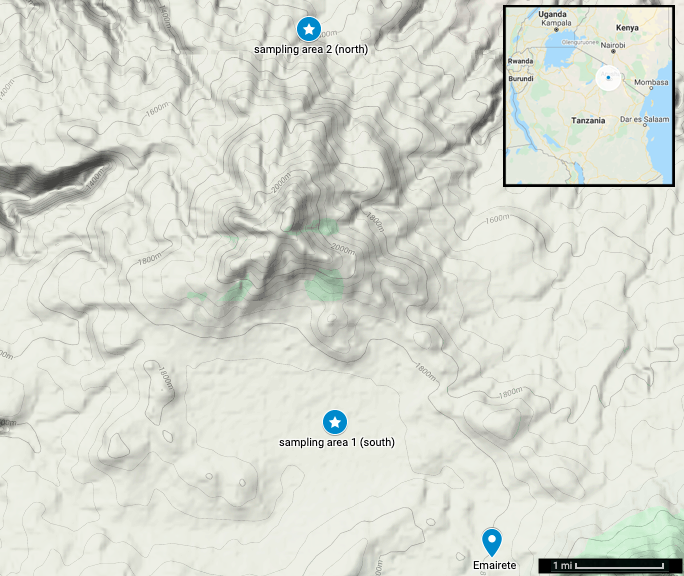
\includegraphics[width=0.9\linewidth,height=0.9\textheight]{images/eluwai-terrain-map} 

}

\caption{Eluwai village area with terrain image showing the approximate center of sampling area 1 (southern region) and sampling area 2 (northern region), both of which are separated by a small mountain (center). Emairete town neighbors the south of sampling area 1, and is connected by paved road to a larger town, Monduli Chini, which is slightly further south (not included in this map). Inset: Map of Tanzania showing the approximate location of the fieldsite in northern Tanzania (blue point, encircled in white).}\label{fig:eluwaimap}
\end{figure}

\hypertarget{methods}{%
\section{Methods}\label{methods}}

Data collection involved structured surveys and a trust vignette
experiment with adult Kisongo Maasai pastoralists (\(N=225\); \(41\%\)
female, \(59\%\) male) in both northern (\(N=141\)) and southern
(\(N=84\)) regions of Eluwai. Surveys in the southern region were
collected by A.D.L. with assistance from a Maasai translator, and by an
additional local Maasai research assistant. Surveys in the northern
region were collected by another local Maasai research assistant. Both
research assistants have more than ten years of experience administering
surveys to local populations, and were trained to conduct the survey by
A.D.L. Data were collected January through March 2020. Interviews took
about 30 minutes. Each participant was paid 10,000 Tanzanian Shillings
(about \$4.35 USD) for their participation (about the price of lunch at
a local restaurant). All preregistered predictions, models, and analysis
scripts can be found at \url{https://osf.io/5p7ut}. All protocols and
survey materials were approved by Washington State University IRB and
Tanzanian Commission for Science and Technology (COSTECH) prior to data
collection.

\hypertarget{study-design}{%
\subsection{Study design}\label{study-design}}

To test the PBM and RIM, we conducted a vignette experiment in which a
hypothetical person from the community describes an inconveniently
faraway location (about a day walking), where he says the participant
should move their livestock to find plenty of available grass and water.
The advice presents a conundrum: Should the participant trust the advice
and act on it? Should they be skeptical and fact-check it first? Should
they reject the advice altogether? If the advice is accepted, then it
would lead to a large benefit if true, but a large cost if false. If it
is rejected, then it would be an opportunity cost if true, but avoid a
large cost if false. If the advice is fact-checked before acting on it,
then a smaller cost is taken on to reduce the risk of accepting the
advice and acting on
it.\footnote{In the literature on the evolution of social learning, asocial learning is (\emph{a priori}) more costly than social learning. It is worth emphasizing that our study does not compare social to asocial learning. Instead, it compares social to state-dependent learning, with asocial learning as one of our two outcomes (i.e., the “fact-checking” outcome variable), consistent with the literature we cite on trust. In other words, \emph{given social learning}, what predicts trust -- prestige or state?}

Each participant was randomly assigned to either a \emph{prestige}
condition or a \emph{participant experience} condition. In the prestige
condition (\(N=113\)) the source of advice was described as a person
with high levels of \emph{nkanyit}, an important Maasai prestige concept
that translates in Maa to ``respect'', but also has connotations of fear
and deference, cattle wealth, and indisputable authority (Spencer 1965,
1988). To confirm these connotations, we asked a subset of our
participants to freelist what gives a person nkanyit. The most salient
responses included cattle weath, caring for a large family, having good
moral character, helping others, and being knowledgeable (see the SI).
Consistent with the assumptions in our study design, informants also
emphasized that although nkanyit can imply knowledge, knowledge does not
imply nkanyit.

Prestige bias theorists argue that cues of prestige can be more reliable
than ``gradually learning via individual experience who the most
successful, knowledgeable, or skillful individuals are'' (J Henrich et
al., 2001, p. 345). In the participant experience condition (\(N=107\))
the source of advice was therefore described as someone the participant
has known from personal experience to be generally
knowledgeable.\footnote{Our use of the term \emph{experience} refers to the participant's experience that the fictional advisor is generally knowledgeable, and does not imply that the fictional advisor actually has experience of the grazing conditions that he is describing.}

Participants were then asked how much they trusted the advice, and
whether or not they would fact-check it first (i.e., personally visit
before taking their livestock there). A more comprehensive structured
survey was then conducted (described below). It is worth noting that in
neither condition was the fictional source of advice described as having
specific or direct knowledge of grazing conditions. See the SI for
complete vignette text and nkanyit freelist data.

\hypertarget{measures}{%
\subsection{Measures}\label{measures}}

\hypertarget{experimental-outcomes}{%
\subsubsection{Experimental outcomes}\label{experimental-outcomes}}

Our two post-intervention outcome variables were \emph{trust} (stated
level of belief that the advice given is true) and \emph{fact-checking}
(if the participant would verify the advice before acting on it). Trust
outcomes were coded on a three-point scale (1 = completely trust, 0.5 =
somewhat trust, 0 = does not trust). Fact-checking outcomes were
measured as simple yes/no responses (1 = yes, 0 = no). See the
preregistration \url{https://osf.io/5p7ut} and section 3 of the SI for
details.

\hypertarget{observational-measures-for-preregistered-tests}{%
\subsubsection{Observational measures for preregistered
tests}\label{observational-measures-for-preregistered-tests}}

Household-level resource scarcity was based on food insecurity scores
and a proxy measure of household need. Food insecurity scores were
determined by a modified 5-item version of a standard 6-item household
food insecurity survey, where higher values indicate higher insecurity
(Blumberg, Bialostosky, Hamilton, \& Briefel, 1999). (Prior to data
collection, a question about diet breadth was removed because it did not
make sense for participants in this region, where narrow diets of milk
and meat are ideal.) Household need was approximated using
consumer-to-producer ratios (i.e., total number of people living in the
household, divided by people reported to regularly contribute to
subsistence in the household; more consumers per producer implied higher
need). Measures of household wealth were based on an index consisting of
three reliable wealth indicators in the region: presence/absence of a
solar panel (1 = presence, 0 = absence), roof material (1 = metal, 0 =
grass), and number of wives in the household. To measure how dependent a
household was on livestock, we collected a list of the different ways
people in the household made a living, using freelists and prompted
options with yes/no responses. Prompts were livestock, farming,
milk/meat sales, crop sales, handcraft sales, wage labor, owning a
business, teaching, and other (if yes, specify). Dependence on livestock
was then estimated by dividing presence/absence of herding livestock for
subsistence (1 = yes, 0 = no) by the total number of subsistence sources
listed, creating a proportion of livelihood strategies involving
livestock (1 = completely dependent on livestock, 0 = not dependent on
livestock at all).

\hypertarget{exploratory-measures}{%
\subsubsection{Exploratory measures}\label{exploratory-measures}}

Our survey included several measures across two domains -- ideational
and material -- for which we had no preregistered hypotheses. Measures
of traditional beliefs (TB) included cultural values, such as religious
beliefs and practices, e.g., religious affiliation, frequency of prayer
(coded on a ranked scale between 1 = never and 5 = very often), and
beliefs about god's characteristics. Whether or not god punishes
misbehavior; rewards good behavior; and is omniscient, omnibenevolent,
and/or omnipotent were each measured as yes (1), no (-1), or don't know
(0). Cultural values involved agree/disagree responses to divisive
statements that are rooted in traditional Maasai ideals. Traditionally
agreeable statements include: females should be circumcised, all cattle
in the world rightfully belong to Maasai people, it is acceptable to
raid cattle from people who are not Maasai, and it is ideal for elder
men to have multiple wives; a disagreeable statement includes: it is
acceptable for women to see a warrior eat meat. Traditionally neutral
statements held mostly by Christians in the region include: belief in
god is the most important thing in life, and women and children should
be educated in school (e.g., Jacobs, 1965; Hodgson, 1999; Spear \&
Waller, 1993; Spencer, 1965). Responses to each statement in the
cultural values survey were measured as strongly agree (2), agree (1),
no opinion (0), disagree (-1), strongly disagree (-2).

Material domains included an \emph{a priori} index of market integration
(MI) to approximate frequency of cash sales and purchases, based on how
often people made purchases at the market (coded on a ranked scale
between 1 = never and 5 = very often), whether or not participants sold
handcrafts, crops, and/or dairy products at markets (0 = no, 1 = yes for
each), and frequency of cell phone use (1 = never, 2 = sometimes, 3 =
often), yielding an index range of 2-10. Measures also included level of
education (0 = none, 1 = primary, 2 = secondary) and literacy (0 = no, 1
= yes). Herd size and composition (e.g., cattle, sheep, goats, donkeys,
and chickens) were self-reported and also included as tropical livestock
units (TLU), an estimate of livestock resources based on grazing
capacity (Jahnke \& Jahnke, 1982).

Although our use of nkanyit as a prestige cue was motivated by prior key
informant interviews and existing literature (e.g., Spencer, 1965,
2004a, 2004b), we also collected freelist data (\(N=57\)) about nkanyit
to validate this choice. See SI for details.

\hypertarget{confirmatory-analyses}{%
\subsection{Confirmatory analyses}\label{confirmatory-analyses}}

We tested our predictions using separate sets of logistic regression
models for the PBM and the RIM, as specified in our preregistration,
with \(\alpha=0.05\). For the strong version of the PBM, our independent
variable was the vignette condition only (\(VC\): 0 = experience, 1 =
prestige). To adhere to our preregistration, we modeled both outcomes
using logistic regression, despite the trust outcome being on a
three-point scale (0, 0.5, and 1; see Britt \& Weisburd (2010) and the
SI where we fit ordinal regression models). We predicted a statistically
significant positive coefficient for \(VC\) for the trust outcome, and a
statistically significant negative coefficient for the fact-checking
outcome:

\[
\begin{aligned}
\text{logit(trust)} = \beta_0 + \beta_{1}VC, \text{where we predicted } \beta_1 > 0 \\
\text{logit(check)} = \beta_0 + \beta_{1}VC, \text{where we predicted } \beta_1 < 0
\end{aligned}
\]

For the RIM, our independent variables were food insecurity scores
(\(F\)), household need (\(N\)), wealth (\(W\)), and dependence on
livestock (\(D\)) for subsistence. We predicted that for trust outcomes
aggregated across conditions (i.e., ignoring any effect of \(VC\)), we
would find statistically significant positive coefficients for \(F\) and
\(N\), and statistically significant negative coefficients for \(W\) and
\(D\). We predicted these coefficients to be reversed for fact-checking
outcomes:

\[
\begin{aligned}
\text{logit(trust)} = \beta_0 + \beta_{1}F + \beta_{2}N +\beta_{3}W +\beta_{4}D, \text{where we predicted } \beta_1, \beta_2 < 0, \text{and } \beta_3, \beta_4 > 0 \\
\text{logit(check)} = \beta_0 + \beta_{1}F + \beta_{2}N +\beta_{3}W +\beta_{4}D, \text{where we predicted } \beta_1, \beta_2 > 0, \text{and } \beta_3, \beta_4 <  0
\end{aligned}
\]

We then compared the PBM, RIM, and PBM+RIM (PBM+RIM was the RIM models
with an additional term for \(VC\), which corresponds to the weak
version of the PBM) using the corrected Akaike information criterion
(AICc), preferring the model with the lowest AICc value (Burnham \&
Anderson, 2004).

\hypertarget{exploratory-analyses}{%
\subsection{Exploratory analyses}\label{exploratory-analyses}}

Prior to fieldwork, we anticipated cultural and economic variation would
be associated with different response patterns but did not know how it
would be distributed. To explore covariation of all diverse variables
characterizing sociodemographic, economic, and ideational aspects of
participants in our dataset, we conducted a principal components
analysis (PCA) on all quantitative observational measures on households
and participants for which there were 10 or fewer missing values,
resulting in 53 measures across all domains in the survey. If the
principal components were interpretable, we aimed to test if one or more
of them was associated with our \emph{trust} and \emph{fact-checking}
outcomes. (The PCA excluded both outcome variables, region, and
experimental condition.)

To use data from all participants, we imputed missing values using the
\emph{mice} package (van Buuren \& Groothuis-Oudshoorn, 2011) for
multiple imputation by chained equations (MICE; Azur et al.~2011), with
the default predictive mean matching method for numeric and logistic
regression for binary variables. MICE assumes that data are missing at
random (MAR). That is, after controlling for all other variables in the
study, any remaining missingness is completely random. All exploratory
results, including the PCA, are pooled estimates from five imputed
datasets (Rubin, 1988). See the SI for a walkthrough of variable
selection, multiple imputation processes, and quality checks on imputed
datasets. (Because we did not preregister imputation, we did not use it
for the confirmatory analyses.) Two participants had extremely high
numbers of children, which had an undue influence on the PCA, and were
therefore removed from the exploratory analyses.

\hypertarget{results}{%
\section{Results}\label{results}}

\hypertarget{cultural-and-regional-variation}{%
\subsection{Cultural and regional
variation}\label{cultural-and-regional-variation}}

Summary statistics are in table 1. PCA results showed systematically
different response patterns corresponding to ideational, material, and
regional variation around Eluwai. The variables with high negative
loadings on PC1 exclusively represented adherence to traditional Maasai
ideals, beliefs and material practices (large herds; high dependence on
livestock; approval of cattle raiding, female circumcision, and
polygyny; and agreement with traditional Maasai beliefs about cattle
ownership). The variables with high positive loadings on PC1 represented
adherence to more recently introduced ideals, beliefs and material
behaviors, such as crop sales, farming, higher education, literacy,
handcraft sales, and prayer frequency (prayer frequency is generally
higher among Christians, mean = 3.6, than among traditional Maasai
believers, mean = 2.5; \(t=\) 5.1, \(p=\) \(\ensuremath{10^{-6}}\)). PC2
reflected household size. See figure 2A.

We therefore interpret PC1 as a latent \emph{acculturation} variable
corresponding to \emph{both} ideational and material changes in the area
(e.g., market integration, missionization, education). Ideational and
material variation along PC1 largely mapped onto regional variation,
such that participants living north of the mountain clustered along the
lower end of PC1 (more traditional) and participants living south of the
mountain (near town, markets, churches, paved roads, and schools)
clustered along the higher end of PC1 (more acculturated). See figure
2B. We found no meaningful sex differences in our PCA results. See SI
for details.

\begin{landscape}

\begin{table}
\caption{\label{tab:summary_tab}Summary statistics for most of the quantitative and ranked observations data used in this study. This includes data used to model and  test our study predictions, but also includes descriptive variables about the sample and a few key variables systematically varying across different regions of the field site. Trust and check refer to our two outcome variables, and food insecurity, household need, wealth, and dependence on cattle were used as observed predictors. Excluding both outcome variables, each variable showed here was included in the PCA described in this section.}

\centering
\fontsize{9}{11}\selectfont
\begin{tabular}{lrrrll}
\toprule
name & complete & mean & sd & range & histogram\\
\midrule
age & 0.99 & 42.3 & 16.0 & 19 - 80 & ▆▇▅▁▃\\
wives & 0.98 & 2.3 & 2.0 & 0 - 12 & ▇▂▁▁▁\\
children & 0.98 & 6.5 & 6.8 & 0 - 40 & ▇▂▁▁▁\\
literate & 0.99 & 0.2 & 0.4 & 0 - 1 & ▇▁▁▁▂\\
education & 0.99 & 1.3 & 0.5 & 1 - 3 & ▇▁▂▁▁\\
\addlinespace
sells dairy & 0.98 & 0.1 & 0.3 & 0 - 1 & ▇▁▁▁▁\\
sells handcrafts & 0.98 & 0.1 & 0.3 & 0 - 1 & ▇▁▁▁▁\\
wage labor & 0.98 & 0.1 & 0.3 & 0 - 1 & ▇▁▁▁▁\\
farms & 0.98 & 0.8 & 0.4 & 0 - 1 & ▂▁▁▁▇\\
sells crops & 0.98 & 0.4 & 0.5 & 0 - 1 & ▇▁▁▁▆\\
\addlinespace
owns a business & 0.98 & 0.2 & 0.4 & 0 - 1 & ▇▁▁▁▂\\
teaches & 0.98 & 0.0 & 0.2 & 0 - 1 & ▇▁▁▁▁\\
household size & 0.98 & 9.2 & 10.8 & 1 - 105 & ▇▁▁▁▁\\
household labor & 0.98 & 4.5 & 8.7 & 1 - 100 & ▇▁▁▁▁\\
freq. urban travel & 0.99 & 1.8 & 1.1 & 1 - 5 & ▇▃▂▁▁\\
\addlinespace
Engai/Christian same & 1.00 & 0.6 & 0.7 & -1 - 1 & ▂▁▂▁▇\\
god has a mind & 0.99 & 0.2 & 0.8 & -1 - 1 & ▅▁▆▁▇\\
god has a body & 0.99 & -0.2 & 0.8 & -1 - 1 & ▇▁▇▁▃\\
god omnipotent & 0.99 & 0.8 & 0.5 & -1 - 1 & ▁▁▁▁▇\\
god omniscient & 1.00 & 0.8 & 0.5 & -1 - 1 & ▁▁▁▁▇\\
\addlinespace
god omnibenevolent & 0.99 & 0.8 & 0.6 & -1 - 1 & ▁▁▁▁▇\\
god punishes & 0.99 & 0.3 & 0.7 & -1 - 1 & ▂▁▇▁▇\\
god rewards & 0.98 & 0.5 & 0.6 & -1 - 1 & ▁▁▆▁▇\\
freq. church/rituals & 0.97 & 2.1 & 1.4 & 1 - 5 & ▇▂▁▃▁\\
freq. prayer & 0.96 & 3.1 & 1.6 & 1 - 5 & ▆▁▁▇▃\\
\addlinespace
freq. talk abt. god & 0.96 & 1.5 & 1.1 & 1 - 5 & ▇▁▁▁▁\\
Maasai cattle rights & 1.00 & 0.8 & 1.3 & -2 - 2 & ▁▅▁▅▇\\
\bottomrule
\end{tabular}
\centering
\begin{tabular}{lrrrll}
\toprule
name & complete & mean & sd & range & histogram\\
\midrule
polygyny & 1.00 & 0.8 & 1.1 & -2 - 2 & ▁▂▁▇▅\\
warrior food taboos & 0.98 & -0.5 & 1.2 & -2 - 2 & ▂▇▂▁▂\\
cattle raiding & 0.96 & -0.1 & 1.3 & -2 - 2 & ▂▇▃▅▃\\
educate children & 1.00 & 1.2 & 0.9 & -2 - 2 & ▁▁▂▇▇\\
educate women & 0.97 & 0.9 & 1.0 & -2 - 2 & ▁▁▂▇▅\\
\addlinespace
cattle > cash & 0.99 & 0.7 & 1.1 & -2 - 2 & ▁▅▆▇▇\\
belief in god is important & 0.98 & 1.0 & 0.9 & -2 - 2 & ▁▁▂▇▅\\
children share religion & 0.98 & 0.9 & 1.0 & -2 - 2 & ▁▂▃▇▆\\
people share religion & 0.98 & 0.8 & 1.0 & -2 - 2 & ▁▂▃▇▅\\
farm for most food & 0.99 & 1.0 & 0.9 & -2 - 2 & ▁▁▂▇▅\\
\addlinespace
female circumcision & 0.98 & 0.3 & 1.3 & -2 - 2 & ▁▇▃▆▆\\
worry about future of Maasai & 0.96 & 0.3 & 1.1 & -2 - 2 & ▁▅▃▇▃\\
god gives comfort/safety & 0.99 & 1.1 & 0.9 & -2 - 2 & ▁▁▂▇▆\\
donkeys & 0.98 & 6.0 & 11.7 & 0 - 92 & ▇▁▁▁▁\\
chickens & 0.99 & 5.3 & 19.0 & 0 - 250 & ▇▁▁▁▁\\
\addlinespace
cattle & 0.98 & 34.7 & 90.6 & 0 - 1000 & ▇▁▁▁▁\\
goats & 0.97 & 32.5 & 67.3 & 1 - 750 & ▇▁▁▁▁\\
sheep & 0.97 & 26.4 & 59.6 & 0 - 520 & ▇▁▁▁▁\\
metal roof & 1.00 & 0.2 & 0.4 & 0 - 1 & ▇▁▁▁▂\\
solar panel & 0.97 & 0.3 & 0.4 & 0 - 1 & ▇▁▁▁▃\\
\addlinespace
market integration & 0.96 & 4.1 & 1.2 & 1 - 7 & ▁▇▆▅▃\\
food insecurity & 1.00 & 1.0 & 0.4 & 0 - 1.75 & ▁▁▇▅▂\\
household need & 0.97 & 2.6 & 1.8 & 1 - 20 & ▇▁▁▁▁\\
dependence on livestock & 0.97 & 0.5 & 0.2 & 0 - 1 & ▂▇▆▁▂\\
freq. cash purchases & 0.99 & 3.5 & 0.7 & 1 - 5 & ▁▂▇▇▁\\
\addlinespace
trust & 0.97 & 0.3 & 0.4 & 0 - 1 & ▇▁▁▁▃\\
fact-check & 0.92 & 0.8 & 0.4 & 0 - 1 & ▂▁▁▁▇\\
\bottomrule
\end{tabular}
\end{table}

\end{landscape}

\begin{figure}[H]

{\centering 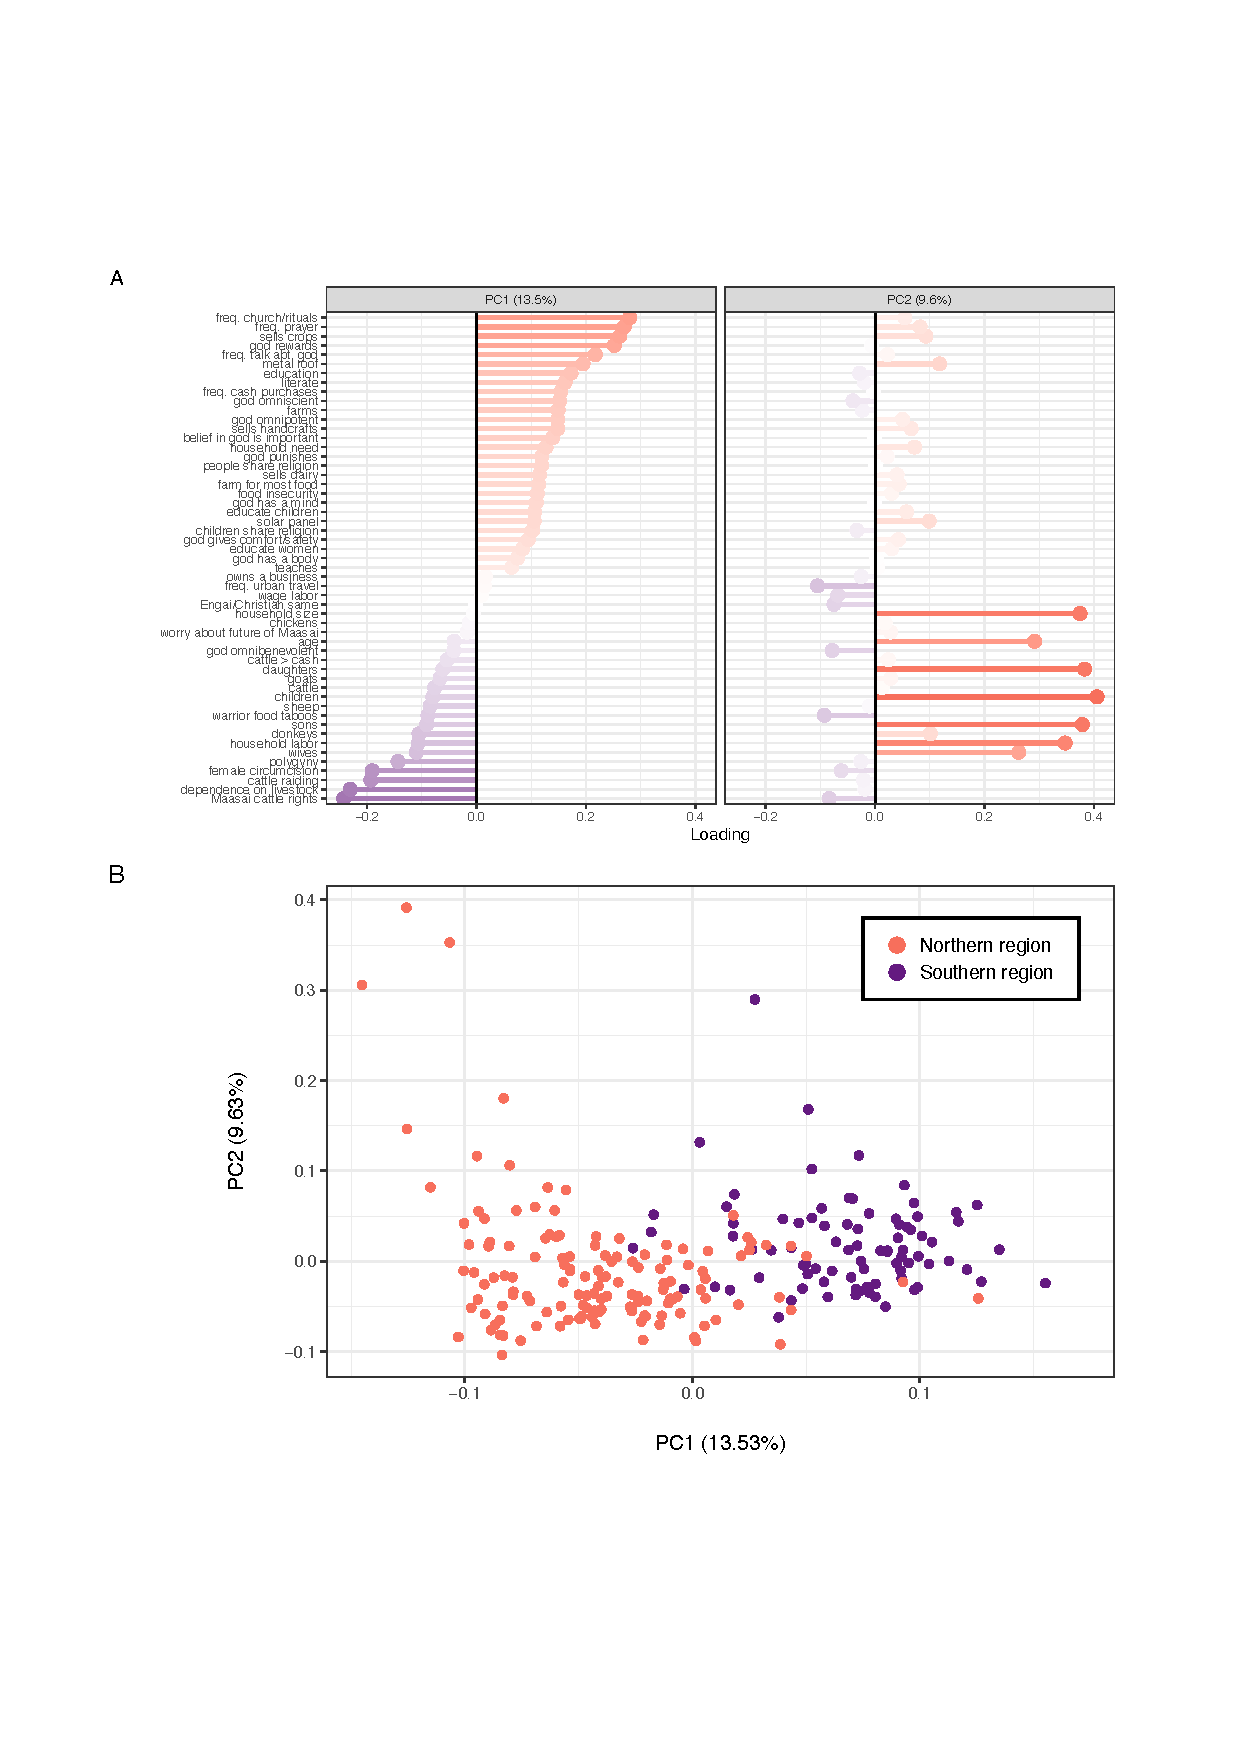
\includegraphics[width=0.9\linewidth]{images/figure2-maintext} 

}

\caption{A: PCA loadings on PC1 and PC2, after including 53 quantitative variables from diverse domains in our analysis. PC1 corresponds to a latent variable characterizing acculturation vs. traditional practices and beliefs. PC2 corresponds to a latent variable characterizing household size. B: PCA biplot, with each point representing one participant. Point colors correspond to participant region.}\label{fig:pcaplot}
\end{figure}

\hypertarget{confirmatory-analyses-testing-the-pbm-and-rim}{%
\subsection{Confirmatory analyses: testing the PBM and
RIM}\label{confirmatory-analyses-testing-the-pbm-and-rim}}

In both the vignette prestige condition and the experience condition,
advice was treated with strong levels of skepticism (experience
condition: 32\% did not trust, 5.5\% somewhat trusted, and 11\%
completely trusted; prestige condition: 33\% did not trust, 4.6\%
somewhat trusted, and 14\% completely trusted), and most participants
stated that they would fact-check the advice before acting on it (86\%
in the experience condition, 82\% in the prestige condition). Thus,
participants had approximately equal, but low, trust for advice from
both the prestigious individual and from the individual known to be
knowledgeable from personal experience.

In our confirmatory analyses for trust outcomes, the RIM was supported
(see table 2 for logistic regression model parameters and statistics,
and figure 3 for RIM effects plots). AICc model selection suggested that
the RIM had better support than the PBM (strong version) and PBM+RIM
(weak
version).\footnote{We re-ran trust models using an ordered logistic regression and found similar effects in each of our models.}
See the SI for additional analyses and weighted AICc table.

\begin{figure}
\centering
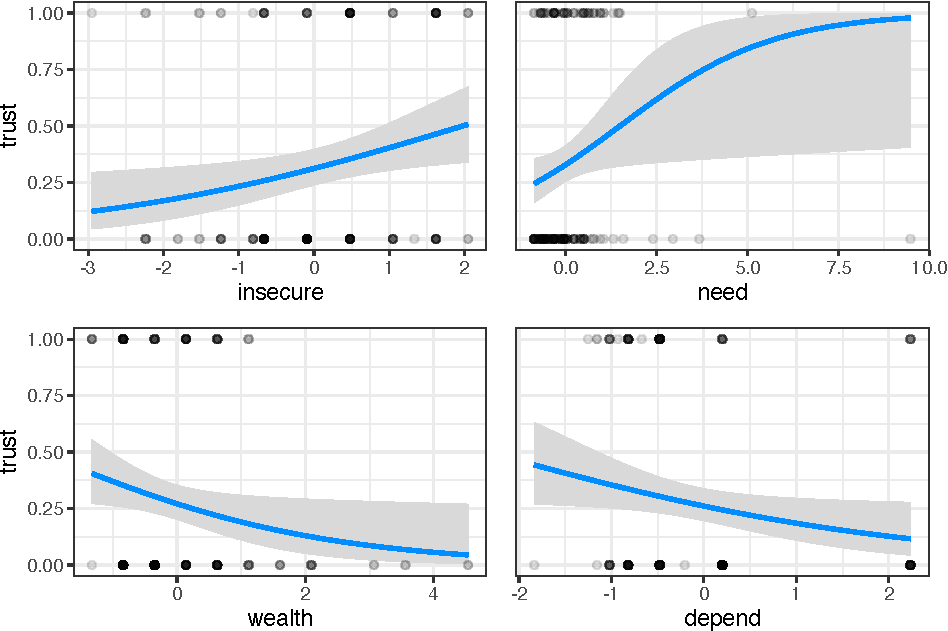
\includegraphics{trust-advice-writeup_files/figure-latex/confirm_effplot-1.pdf}
\caption{Logistic regression models for RIM predictors on trust
outcomes. Model coefficients are in table 2 (column 2).}
\end{figure}

\begin{table}[!htbp] \centering 
  \caption{Logistic regression models for trust outcomes (left three models) and fact-checking outcomes (right three models) based on condition, and on scaled measures of household food insecurity, need, wealth, and dependence on livestock as a source of subsistence. Estimates are log odds, with standard error in parentheses. For each outcome variable, output is shown for preregistered models PBM, RIM, and PBM+RIM.} 
  \label{} 
\begin{tabular}{@{\extracolsep{5pt}}lcccccc} 
\\[-1.8ex] & \multicolumn{6}{c}{\textit{Dependent variable:}} \\ 
\cline{2-7} 
\\[-1.8ex] & \multicolumn{3}{c}{trust} & \multicolumn{3}{c}{check} \\ 
 & PBM & RIM & PBM+RIM & PBM & RIM & PBM+RIM \\ 
\hline \\[-1.8ex] 
 conditionprestige & 0.11 &  & 0.22 & $-$0.32 &  & $-$0.52 \\ 
  & (0.30) &  & (0.35) & (0.38) &  & (0.42) \\ 
  & p = 0.70 &  & p = 0.53 & p = 0.41 &  & p = 0.22 \\ 
  & & & & & & \\ 
 insecure &  & 0.40 & 0.40 &  & $-$0.16 & $-$0.15 \\ 
  &  & (0.17) & (0.17) &  & (0.20) & (0.20) \\ 
  &  & p = 0.02$^{*}$ & p = 0.02$^{*}$ &  & p = 0.43 & p = 0.45 \\ 
  & & & & & & \\ 
 need &  & 0.48 & 0.45 &  & 0.08 & 0.12 \\ 
  &  & (0.23) & (0.23) &  & (0.21) & (0.23) \\ 
  &  & p = 0.04$^{*}$ & p = 0.05$^{*}$ &  & p = 0.70 & p = 0.62 \\ 
  & & & & & & \\ 
 wealth &  & $-$0.46 & $-$0.45 &  & 0.30 & 0.28 \\ 
  &  & (0.22) & (0.22) &  & (0.25) & (0.25) \\ 
  &  & p = 0.04$^{*}$ & p = 0.05$^{*}$ &  & p = 0.23 & p = 0.26 \\ 
  & & & & & & \\ 
 depend &  & $-$0.44 & $-$0.47 &  & 0.36 & 0.44 \\ 
  &  & (0.21) & (0.22) &  & (0.26) & (0.27) \\ 
  &  & p = 0.04$^{*}$ & p = 0.04$^{*}$ &  & p = 0.17 & p = 0.11 \\ 
  & & & & & & \\ 
\hline \\[-1.8ex] 
\textit{Note:}  & \multicolumn{6}{r}{$^{*}$p$<$0.05; $^{**}$p$<$0.01; $^{***}$p$<$0.001} \\ 
\end{tabular} 
\end{table}

\hypertarget{exploratory-analyses-1}{%
\subsection{Exploratory analyses}\label{exploratory-analyses-1}}

\hypertarget{regional-variation-at-the-field-site}{%
\subsubsection{Regional variation at the field
site}\label{regional-variation-at-the-field-site}}

We interpreted PC1 (figure 2) to be a latent acculturation variable,
which was systematically lower in the northern region and higher in the
southern region. Responses in the northern vs.~southern regions varied
on trust outcomes (north: 1 = 51\%, 0.5 = 24\%, 0 = 25\%; south: 1 =
7.8\%, 0.5 = 1.4\%, 0 = 86\%) and fact-checking outcomes (north: 1 =
69\%, 0 = 31\%; south: 1 = 92\%, 0 = 8\%). See figure S7. We therefore
modeled each outcome variable as a function of PC1. Consistent with
regional patterns, more acculturated participants were more likely to
trust livestock advice and less likely to fact-check it, whereas less
acculturated participants were less likely to trust and more likely to
fact-check (figure 4).

\begin{figure}
\centering
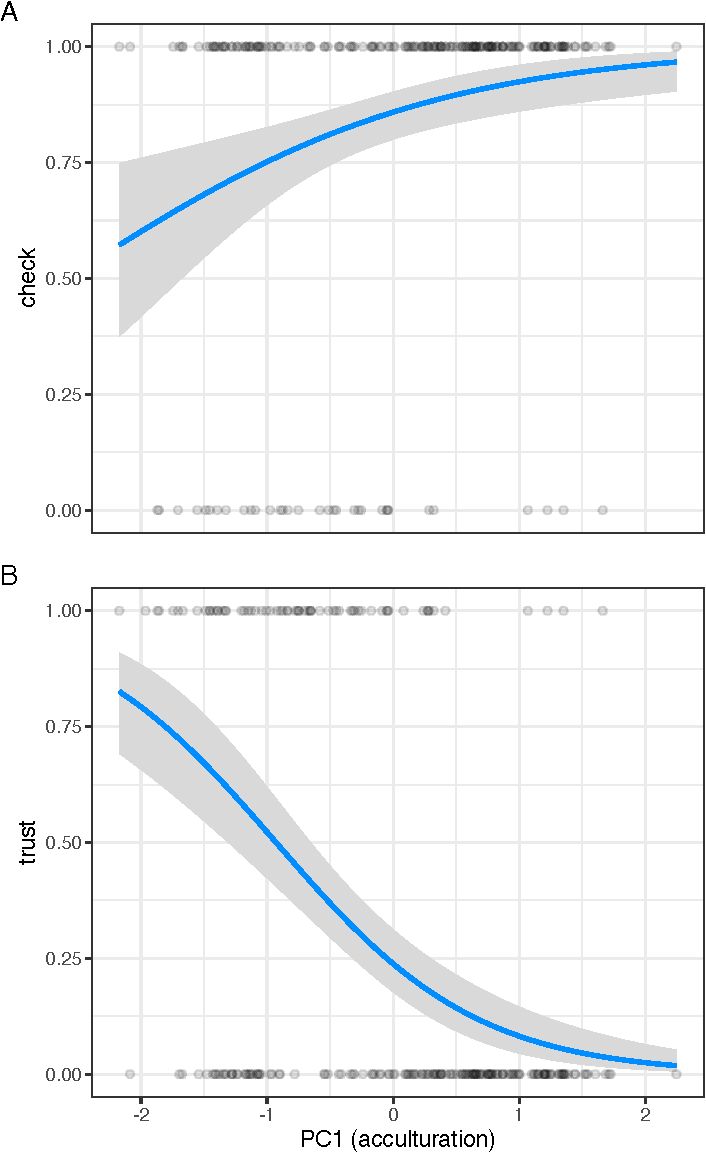
\includegraphics{trust-advice-writeup_files/figure-latex/pca_effplot-1.pdf}
\caption{Fact-checking outcomes (A) and trust outcomes (B) predicted by
PC1, the acculturation variable characterizing response patterns along
the northern vs.~southern sampling areas. Higher levels of PC1
correspond to higher levels of acculturation, such as Christianization
and market integration. Lower levels of PC1 correspond to lower levels
of acculturation, or traditional Maasai beliefs and economic practices.}
\end{figure}

\hypertarget{hierarchical-cluster-analysis}{%
\subsubsection{Hierarchical cluster
analysis}\label{hierarchical-cluster-analysis}}

Variables belonging to both ideational and material categories had high
loadings on PC1 (figure 2a), which in turn distinguished the northern
and southern regions (figure 2b). To explore if response patterns
naturally formed ideational vs.~material clusters, we conducted a
hierarchical cluster analysis using the Ward agglomeration method, with
distances as \(1-corr\), and cluster p-values computed via multiscale
bootstrap resampling (Suzuki, Terada, Shimodaira, \& Suzuki, 2019). We
identified five clusters that were reasonably well-supported by the
bootstrap procedure (\(p > 0.8\)). These were education/urban,
elder/household size, farming/religious, market integration (MI), and
traditional beliefs/large herds (TB). See figure 5. Two of these (TB and
MI) were clearly interpretable as ideational vs.~material. Because we
also developed an \emph{a priori} MI index (see Exploratory measures),
we denote the MI cluster here as \emph{empirically determined MI}
(EMI).\footnote{Note that we made no \emph{a priori} TB index, as we did with MI.}

To explore if material or ideational clusters better predicted trust
than PC1, we used MI, EMI, TB, and dependence on livestock for
subsistence\footnote{We included a model with dependence on livestock (referred to in the RIM as \emph{depend}) because it strongly correlated with PC1, and varied markedly by region. In figure 6, this model is abbreviated as \emph{DEP}.}
each as separate predictors of trust and fact-checking outcomes.
Comparing these models to each other and the confirmatory models, we
found that MI and EMI each predicted higher trust and lower
fact-checking, and while these effects were larger than those in the
RIM, neither were as large as the effect of PC1. Compared to MI, TB
weakly predicted lower trust and higher fact-checking. (Because the
effects of MI and EMI were similar, we refer to them interchangeably in
the Discussion section as ``market integration''.) See figure 6. AICc
model selection consistently suggested across imputations that PC1
models outperformed the other models, including the MI, EMI, TB, depend,
and confirmatory models (table S5). Market integration nevertheless
appeared to have a large impact on trust, compared to adherence to
traditional beliefs and values. See SI for a more detailed discussion.

\begin{figure}
\centering
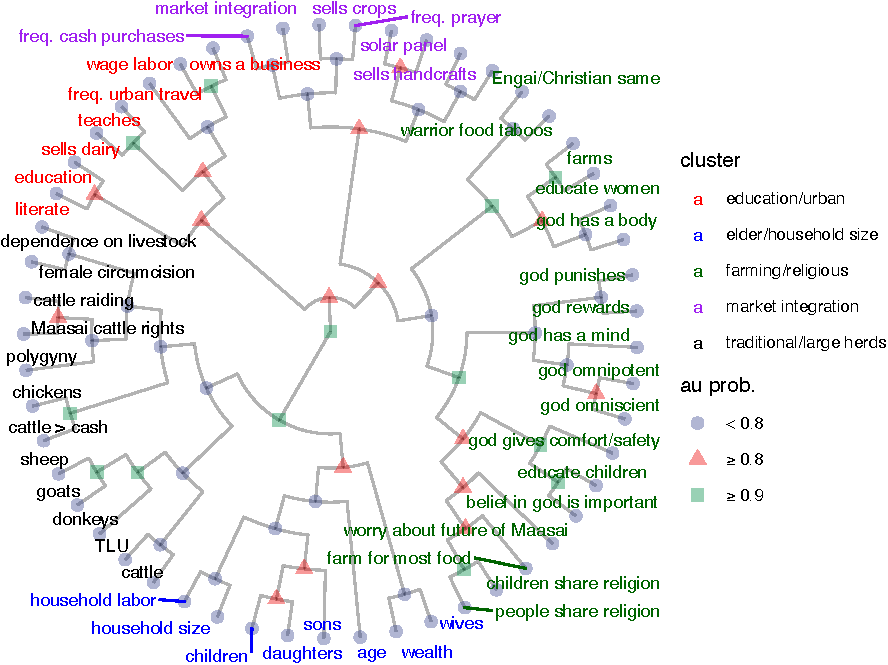
\includegraphics{trust-advice-writeup_files/figure-latex/treeplot-1.pdf}
\caption{Hierarchical clustering dendogram with shapes corresponding to
approximately unbiased (au) branching probabilities (bootstrapped n =
10,000), and colors corresponding to cluster ID. Each cluster is based
in part on au probabilities and our interpretation of cohesive clusters
(e.g., market integration, traditional livelihoods) Some clusters are
less straightforward than others to interpret, but we nevertheless
include a short cluster description next to each color.}
\end{figure}

\begin{figure}
\centering
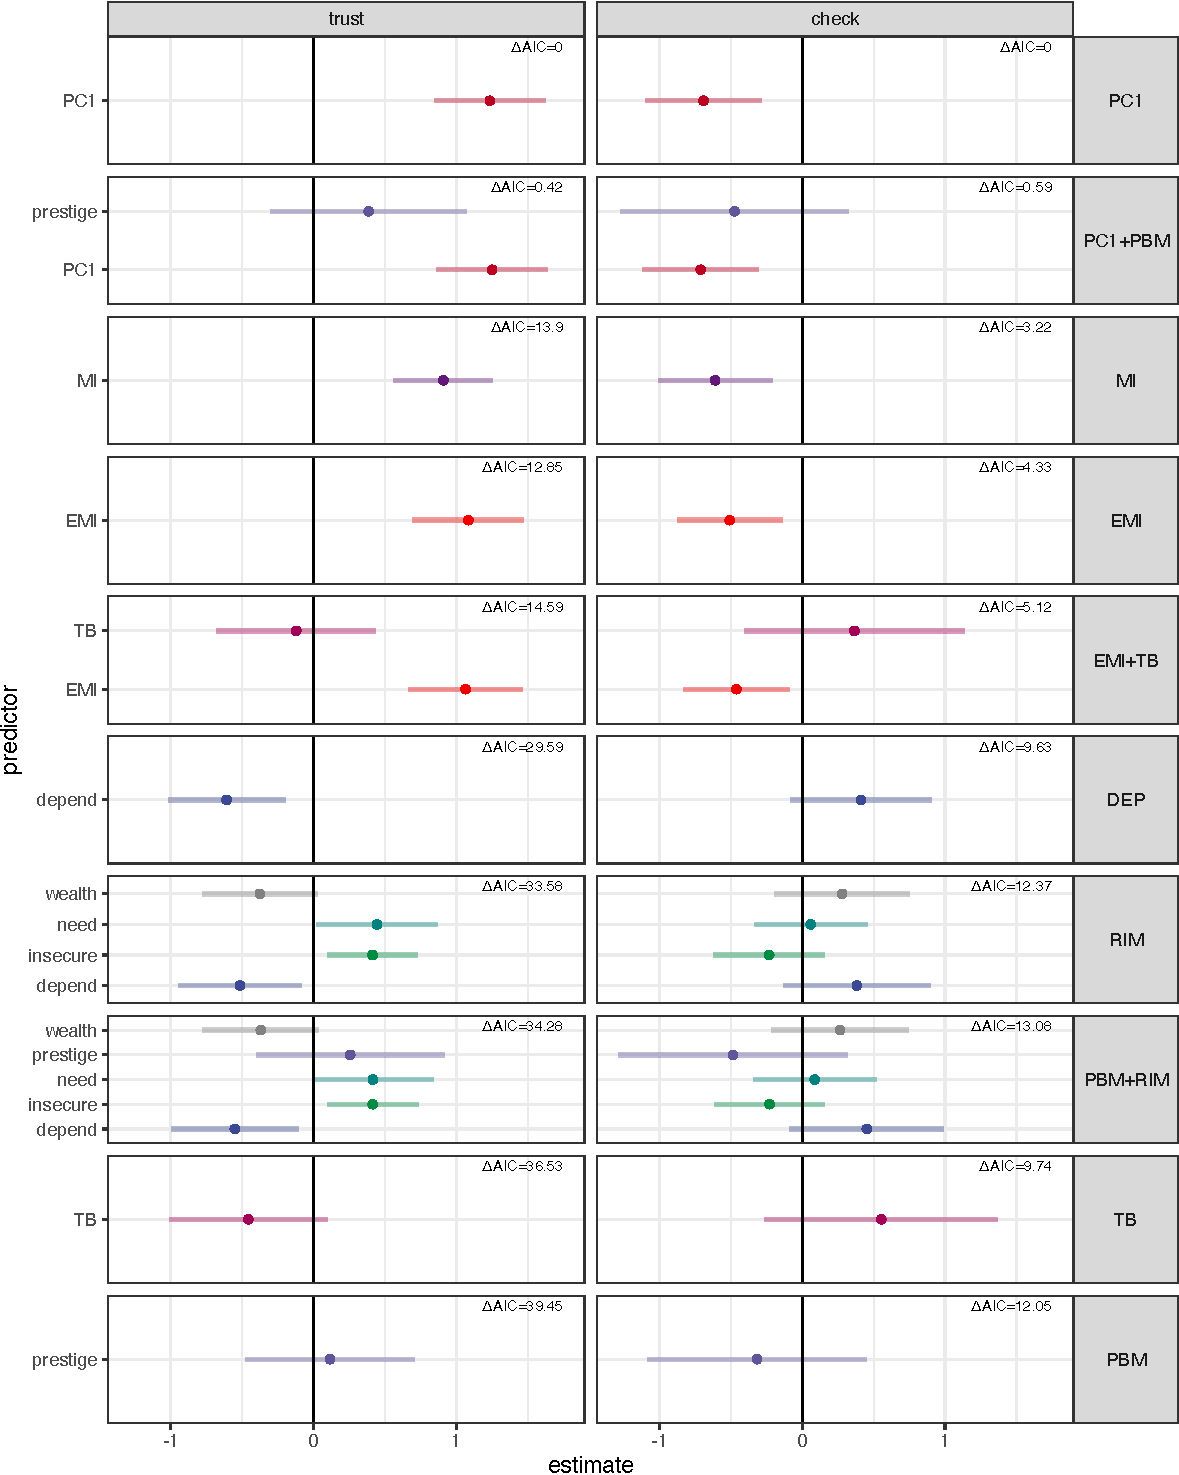
\includegraphics{trust-advice-writeup_files/figure-latex/single_coefficients_plot-1.pdf}
\caption{Coefficients plot for exploratory logistic regression models
predicting trust and fact-checking outcomes. Points indicate regression
coefficients (log odds scale), and error bars are +/- 2 SE. Colors
correspond to different predictors included in various models, whereas
facets separate models included in the model comparison in this section.
Facets are ordered from top to bottom in order of AICc score in weighted
model selection. Tables for this are included in the SI.}
\end{figure}

\newpage

\hypertarget{discussion}{%
\section{Discussion}\label{discussion}}

In a preregistered vignette-based experiment, we tested the roles of
learning biases (PBM) and incentives (RIM) in evaluating socially
learned information about grazing conditions for livestock. The PBM
predicted that if a source of information is prestigious compared to
known from personal experience to be knowledgeable, people would be (1)
more likely to trust and act on their advice, and (2) less likely to
fact-check it first. Neither of these predictions were supported.
Regardless of whether the source was prestigious vs.~believed from
personal experience to be generally knowledgeable, trust in socially
learned information about grazing conditions was equally low in both
conditions, and preferences for fact-checking were also equally high in
both conditions. This lack of support was found when considering
``strong'' and ``weak'' versions of prestige bias (\emph{sensu} Morin
(2016); see Preregistered predictions and Study design sections); we
tested the weak version in PBM+RIM but did not find a statistically
significant effect of prestige (table 1). Nevertheless, 24\% of
participants did trust the fictional advice giver, suggesting that
persons known to be knowledgeable via either their prestige or via
personal experience are trusted to some extent.

The RIM predicted that resource scarce participants who are less
dependent on cattle would be (1) more willing to take a risk and act on
socially learned information, and (2) less likely to fact-check it
first. Prediction 1 was supported, and prediction 2 was not.
Observational measures of resource scarcity (household food insecurity
scores and need) significantly predicted higher trust in, and
willingness to act on, advice about livestock. Conversely, as predicted,
proxy measures of livestock dependence for subsistence and household
wealth predicted lower trust in the same advice. These measures,
however, did not significantly impact participants' stated need to
fact-check before acting on information.

The RIM outperformed the both strong and weak versions of the PBM by
AICc on both trust and fact-checking. See tables 1 and S2. These results
imply that for Maasai in this region, risks and incentives influence
trust about livestock advice, whereas the effect of prestige is
indistinguishable from assessments of knowledgeability based on
participants' personal experiences. More notably, trust and reliance on
social learning, at least for advice about livestock movement, was
generally quite low (see also Toelch, Bruce, Newson, Richerson, \&
Reader, 2014; Mesoudi, Chang, Murray, \& Lu, 2015).

\hypertarget{exploratory-analysis-of-regional-acculturation-as-a-predictor-of-trust}{%
\subsection{Exploratory analysis of regional acculturation as a
predictor of
trust}\label{exploratory-analysis-of-regional-acculturation-as-a-predictor-of-trust}}

Regional acculturation strongly predicted trust. Acculturation was the
first principal component of variables reflecting market integration
vs.~dependence on livestock, and traditional vs.~non-traditional views
about polygyny, female circumcision, and cattle raiding (figure 2). The
study site comprised two distinct regions separated by a small mountain,
with southern, more acculturated participants living closer to densely
populated towns exhibiting higher trust, and northern, less acculturated
participants living on a more rural and isolated side of the mountain
exhibiting lower trust (figures 1 and 4).

To more precisely characterize acculturation, we identified clusters of
variables related to material culture (market integration, MI) and
ideational culture (traditional beliefs, TB). MI was a stronger
predictor of trust than TB, and a model with MI alone outperformed a
model with both, suggesting that MI better explained the strong positive
relationship between regional acculturation and trust. Nevertheless, the
model with acculturation, which reflects covariation among many
variables beyond MI, had the best performance of all (see SI for AICc
tables). This suggests that acculturation was irreducible to either
economic or ecological accounts alone (e.g., Edgerton, 1971). Our
results also suggest that acculturation has a larger influence on
advice-taking than do risks and incentives.

\hypertarget{material-and-ideational-culture}{%
\subsection{Material and ideational
culture}\label{material-and-ideational-culture}}

Material vs.~ideational theories of culture have a long history in
social sciences. Materialist accounts emphasize environmental feedback
and incentive structures: individuals must learn to maximize resources,
and behavioral patterns varying between groups correspond to different
relevant features in the environment (e.g., MI, livelihood risks). If
risk and uncertainty are part of a local subsistence strategy, cultural
adaptations might feature heightened sensitivity to risk (Goldschmidt \&
Goldschmidt, 1976; Steward, 1972). East African pastoralists optimize
herd size and composition (Mace, 1990; Mace \& Houston, 1989; see also
Næss, Bårdsen, Pedersen, \& Tveraa, 2011), and pattern herd movement
based on past and current payoffs (Butt, Shortridge, \& WinklerPrins,
2009; see also Domjan \& Burkhard, 1986).

Ideational accounts, in contrast, emphasize beliefs, attitudes, and
values. Socially transmitted information can establish complex
behavioral conventions (Boyd \& Richerson, 1985; Tennie, Call, \&
Tomasello, 2009), and acculturation can be driven, at least in part, by
novel ideational changes such as religious conversions or
Westernization. In Monduli Juu, missionaries fund organizations that
advocate helping women and children gain access to formal education.
Efforts to convert Maasai to Christianity have largely succeeded, in
part, by appealing to women (Hodgson, 2005) and prioritizing
compatibility with some (but not all) Maasai traditions (Rigby, 1989).
In our data, ideational variables covaried with materialist ones (figure
2).

\hypertarget{conflict-and-coordination-by-region}{%
\subsection{Conflict and coordination by
region}\label{conflict-and-coordination-by-region}}

Land conflicts over grazing are a primary cause of neighbor conflicts
across the broader Monduli Juu region, and large sisal plants now fence
many property lines. This increases resource scarcity (e.g., available
grass) and conflicts of interest among herders. Payoffs to individual
vs.~social learning strongly depend on the accuracy of learning
(McElreath, 2004), and when misinformation is incentivized, the accuracy
of social learning is reduced, and thus so is trust.

Regional variation in trust might reflect different culturally evolved
solutions to a coordination problem (Binmore, 2011; Yamagishi \& Suzuki,
2009), which is mutually compatible with materialist and ideational
accounts. Evidence for this would include low variation within regions,
and sharp discontinuities between regions (Efferson, Vogt, Elhadi,
Ahmed, \& Fehr, 2015; Mackie, 1996). Our data are partially consistent
with this: only 8\% of participants in the north trusted livestock
advice compared to 51\% in the south.

Based on the RIM, which was partially supported, herders should be
skeptical about possibly deceptive advice about their grazing routines
(e.g., Trouche et al., 2018). This is what we observe in the less market
integrated, more cattle dependent northern region. Kinship is an
important criteria for trust among Maasai (Fratkin, 2001; Spencer,
1965), and northern herders might generally mistrust non-kin with
livestock advice -- regardless of prestige or experience. The
advice-giver in the vignette was not specified to be kin (if
participants asked, they were told he was not kin).

In the south, however, trust outcomes were more split. Southern herders
must routinely trust non-kin and distant relatives to successfully
participate in markets. This is a novel coordination problem, because
cash markets and fewer livestock also reduce the scope for land conflict
among herders (see also Cronk \& Leech, 2013). Market-integrated
southern herders might therefore see a demand for ``market norms'',
e.g., expectations for fairness beyond kin groups (J. Henrich et al.,
2010), which can be transmitted socially (Richerson \& Boyd, 2005) or
preferentially attended to by content biases (Cronk, 2017). This account
was particularly well-supported by regional variation in trust outcomes.
Controlling for region, individual incentives did not predict additional
variation in trust, possibly supporting group-level social learning
processes. (Although, as noted here and in figure 2, these incentive
variables were confounded with region.)

Mistrustful southerners might reflect the recent and ongoing nature of
market expansion, infrastructure development, and formal education
(Hodgson, 1999; Swebe, 1984). Multiple small-scale societies, including
a separate Maasai community near Monduli Juu (Baird \& Gray, 2014), saw
disruptions in traditional social conventions after market expansion
(e.g., Ensminger, 1992; Gurven, Jaeggi, von Rueden, Hooper, \& Kaplan,
2015; Kasper \& Borgerhoff Mulder, 2015; North, 1990). Higher livelihood
diversification and lower dependence on cattle could motivate some
southern herders to take strategic risks with their livestock, but
cattle remain common among southern herders. This alone might explain
split trust outcomes, which we did not see in the north. Alternatively,
it is difficult to overstate the importance of cattle to Maasai culture,
regardless of actual subsistence strategy used (Spear \& Waller, 1993).
It is therefore possible that these split trust outcomes near town
result from risk aversion, not due to livelihood risk \emph{per se}, but
to risk to cultural valuation of cattle (see also Herskovits, 1926;
cf.~Dahl \& Hjort, 1976).

\hypertarget{limitations}{%
\subsection{Limitations}\label{limitations}}

This study involved testing preregistered hypotheses using both
experimental and observational study designs. Only one of the
preregistered hypotheses regarding the RIM was supported, with
observational data. Compared to experimental studies, observational
studies provide weak evidence for causality, but allow researchers to
study real-world behaviors that experimental studies usually cannot
(e.g., Hutchins, 2000). Evidence supporting the RIM is therefore
suggestive, and results should be interpreted with caution. Our
vignettes also did not include a condition in which the advice giver was
depicted as unknowledgeable, so we cannot determine if knowledgeability,
inferred from either prestige or personal experience, influences trust.

Although we found clear evidence that acculturation was associated with
trust outcomes, this key finding was not from the preregistered
hypotheses but from \emph{post hoc} exploratory analyses. Exploratory
analyses are especially vulnerable to misinterpreting noise as genuine
signals. Also, data in the northern vs.~southern regions were collected
by different research assistants, raising the possibility that regional
differences in acculturation and trust were somehow a consequence of the
procedures followed by each assistant. Although we cannot completely
rule out an interviewer effect, we doubt it for the following reasons:
both assistants were local adult men with many years of experience
administering surveys. One assistant and A.D.L. separately collected
data in the southern region, and their results were quite similar (i.e.,
a term for interviewer in regression models of data only from the
southern region was not statistically significant; see the SI). Further,
many of the survey items were relatively objective questions involving
roof material, solar panels, number of wives, household size, and so
forth, where interviewer effects would not be expected, and these also
differed systematically by region (see SI for tests of differences by
region).

\hypertarget{conclusion}{%
\subsection{Conclusion}\label{conclusion}}

Socially learned information can imply non-trivial costs and benefits,
including risks of misinformation. Risk and incentives predicted
increased willingness to trust in advice, but prestige did not increase
trust compared to knowledgeability learned from personal experience.
Acculturation, which varied markedly by region, was found to have an
even larger positive association with trust. Much of this effect was due
to the positive effect of market integration on trust, but weaker
adherence to traditional Maasai values was also positively associated
with trust to some degree. The causal pathways among market integration,
acculturation, and trust remain to be clarified.

\hypertarget{acknowledgements}{%
\section{Acknowledgements}\label{acknowledgements}}

We especially thank the Maasai people of Eluwai who participated in this
study. We are also grateful to Musa Kamaika, Kotoke Ngilepoi, and one
anonymous Maasai research assistant for their help during fieldwork. We
thank Anne Pisor, Cynthiann Heckelsmiller, Lee Cronk, Serah Shani, and
two anonymous reviewers for many helpful comments and discussions that
improved this manuscript.

\hypertarget{author-contributions}{%
\section{Author Contributions}\label{author-contributions}}

ADL and EHH designed the study. ADL collected data, and ADL and EHH
analyzed and interpreted data. ADL and EHH wrote the article.

\hypertarget{financial-support}{%
\section{Financial Support}\label{financial-support}}

This project was funded by an NSF Doctoral Dissertation Improvement
Grant (award number 1918523).

\hypertarget{conflicts-of-interest}{%
\section{Conflicts of Interest}\label{conflicts-of-interest}}

The authors declare no conflicts of interest.

\hypertarget{data-availability}{%
\section{Data availability}\label{data-availability}}

All preregistration materials are publicly available at
\url{https://osf.io/5p7ut}. Data are available at
\url{https://doi.org/10.5281/zenodo.4118454}, and supplementary
information and analysis scripts are available at
\url{https://doi.org/10.5281/zenodo.4118474}.

\newpage

\hypertarget{references}{%
\section*{References}\label{references}}
\addcontentsline{toc}{section}{References}

\hypertarget{refs}{}
\leavevmode\hypertarget{ref-2018_JOCCC}{}%
Acerbi, A., \& Tehrani, J. J. (2018). Did Einstein really say that?
Testing content versus context in the cultural selection of quotations.
\emph{Journal of Cognition and Culture}, \emph{18}(3-4), 293--311.

\leavevmode\hypertarget{ref-aokiInstitutionsCognitiveMedia2011}{}%
Aoki, M. (2011). Institutions as cognitive media between strategic
interactions and individual beliefs. \emph{Journal of Economic Behavior
\& Organization}, \emph{79}(1-2), 20--34.
doi:\href{https://doi.org/10.1016/j.jebo.2011.01.025}{10.1016/j.jebo.2011.01.025}

\leavevmode\hypertarget{ref-atkissonAdultLearnersNovel2012}{}%
Atkisson, C., O'Brien, M. J., \& Mesoudi, A. (2012). Adult Learners in a
Novel Environment Use Prestige-Biased Social Learning:
\emph{Evolutionary Psychology}.
doi:\href{https://doi.org/10.1177/147470491201000309}{10.1177/147470491201000309}

\leavevmode\hypertarget{ref-aungerAreFoodAvoidances1994}{}%
Aunger, R. (1994). Are Food Avoidances Maladaptive in the Ituri Forest
of Zaire? \emph{Journal of Anthropological Research}, \emph{50}(3),
277--310.

\leavevmode\hypertarget{ref-axsomAudienceResponseHeuristic1987}{}%
Axsom, D., Yates, S., \& Chaiken, S. (1987). Audience response as a
heuristic cue in persuasion. \emph{Journal of Personality and Social
Psychology}, \emph{53}(1), 30--40.
doi:\href{https://doi.org/10.1037/0022-3514.53.1.30}{10.1037/0022-3514.53.1.30}

\leavevmode\hypertarget{ref-bairdConservationUnscriptedDevelopment2014}{}%
Baird, T. D. (2014). Conservation and Unscripted Development: Proximity
to Park Associated with Development and Financial Diversity.
\emph{Ecology and Society}, \emph{19}(1).

\leavevmode\hypertarget{ref-bairdLivelihoodDiversificationShifting2014a}{}%
Baird, T. D., \& Gray, C. L. (2014). Livelihood Diversification and
Shifting Social Networks of Exchange: A Social Network Transition?
\emph{World Development}, \emph{60}, 14--30.
doi:\href{https://doi.org/10.1016/j.worlddev.2014.02.002}{10.1016/j.worlddev.2014.02.002}

\leavevmode\hypertarget{ref-bellEvolutionaryThinkingMicroeconomic2013}{}%
Bell, A. V. (2013). Evolutionary Thinking in Microeconomic Models:
Prestige Bias and Market Bubbles. \emph{PLOS ONE}, \emph{8}(3), e59805.
doi:\href{https://doi.org/10.1371/journal.pone.0059805}{10.1371/journal.pone.0059805}

\leavevmode\hypertarget{ref-binmoreNaturalJustice2011}{}%
Binmore, K. (2011). \emph{Natural justice}. Oxford: Oxford Univ. Press.

\leavevmode\hypertarget{ref-blumbergEffectivenessShortForm1999a}{}%
Blumberg, S. J., Bialostosky, K., Hamilton, W. L., \& Briefel, R. R.
(1999). The effectiveness of a short form of the Household Food Security
Scale. \emph{American Journal of Public Health}, \emph{89}(8),
1231--1234.

\leavevmode\hypertarget{ref-boesen1976tanzania}{}%
Boesen, J. (1976). \emph{Tanzania-from ujamaa to villagization}.
Institute for Development Research.

\leavevmode\hypertarget{ref-boydCultureEvolutionaryProcess1985}{}%
Boyd, R., \& Richerson, P. J. (1985). \emph{Culture and the evolutionary
process} (Paperback ed.). Chicago (u.a.): University of Chicago Press.

\leavevmode\hypertarget{ref-brandEmergenceAdaptiveUse2020}{}%
Brand, C. O., Heap, S., Morgan, T. J. H., \& Mesoudi, A. (2020). The
emergence and adaptive use of prestige in an online social learning
task. \emph{Scientific Reports}, \emph{10}(1), 12095.
doi:\href{https://doi.org/10.1038/s41598-020-68982-4}{10.1038/s41598-020-68982-4}

\leavevmode\hypertarget{ref-brittLogisticRegressionModels2010}{}%
Britt, C. L., \& Weisburd, D. (2010). Logistic Regression Models for
Categorical Outcome Variables. In A. R. Piquero \& D. Weisburd (Eds.),
\emph{Handbook of Quantitative Criminology} (pp. 649--682). New York,
NY: Springer.
doi:\href{https://doi.org/10.1007/978-0-387-77650-7_31}{10.1007/978-0-387-77650-7\_31}

\leavevmode\hypertarget{ref-burnhamMultimodelInferenceUnderstanding2004}{}%
Burnham, K. P., \& Anderson, D. R. (2004). Multimodel Inference:
Understanding AIC and BIC in Model Selection. \emph{Sociological Methods
\& Research}, \emph{33}(2), 261--304.
doi:\href{https://doi.org/10.1177/0049124104268644}{10.1177/0049124104268644}

\leavevmode\hypertarget{ref-buttEcologyMobilityLabour2016}{}%
Butt, B. (2016). Ecology, mobility and labour: Dynamic pastoral herd
management in an uncertain world. \emph{Revue Scientifique Et Technique
(International Office of Epizootics)}, \emph{35}(2), 461--472.
doi:\href{https://doi.org/10.20506/rst.35.2.2530}{10.20506/rst.35.2.2530}

\leavevmode\hypertarget{ref-buttPastoralHerdManagement2009}{}%
Butt, B., Shortridge, A., \& WinklerPrins, A. M. G. A. (2009). Pastoral
Herd Management, Drought Coping Strategies, and Cattle Mobility in
Southern Kenya. \emph{Annals of the Association of American
Geographers}, \emph{99}(2), 309--334.
doi:\href{https://doi.org/10.1080/00045600802685895}{10.1080/00045600802685895}

\leavevmode\hypertarget{ref-caracoRisksensitivityAmbientTemperature1990}{}%
Caraco, T., Blanckenhorn, W. U., Gregory, G. M., Newman, J. A., Recer,
G. M., \& Zwicker, S. M. (1990). Risk-sensitivity: Ambient temperature
affects foraging choice. \emph{Animal Behaviour}, \emph{39}(2),
338--345.
doi:\href{https://doi.org/10.1016/S0003-3472(05)80879-6}{10.1016/S0003-3472(05)80879-6}

\leavevmode\hypertarget{ref-chudekPrestigebiasedCulturalLearning2012a}{}%
Chudek, M., Heller, S., Birch, S., \& Henrich, J. (2012).
Prestige-biased cultural learning: Bystander's differential attention to
potential models influences children's learning. \emph{Evolution and
Human Behavior}, \emph{33}(1), 46--56.
doi:\href{https://doi.org/10.1016/j.evolhumbehav.2011.05.005}{10.1016/j.evolhumbehav.2011.05.005}

\leavevmode\hypertarget{ref-conwayiiiWhenAuthoritiesCommands2005}{}%
Conway, L. G., \& Schaller, M. (2005). When authorities' commands
backfire: Attributions about consensus and effects on deviant decision
making. \emph{Journal of Personality and Social Psychology},
\emph{89}(3), 311--326.
doi:\href{https://doi.org/10.1037/0022-3514.89.3.311}{10.1037/0022-3514.89.3.311}

\leavevmode\hypertarget{ref-cronkCultureInfluenceBehavior2017a}{}%
Cronk, L. (2017). Culture's influence on behavior: Steps toward a
theory. \emph{Evolutionary Behavioral Sciences}, \emph{11}(1), 36--52.
doi:\href{https://doi.org/10.1037/ebs0000069}{10.1037/ebs0000069}

\leavevmode\hypertarget{ref-cronkMeetingGrandCentral2012}{}%
Cronk, L., \& Leech, B. (2013). \emph{Meeting at Grand Central}.

\leavevmode\hypertarget{ref-curtin2020kinship}{}%
Curtin, C. M., Barrett, H. C., Bolyanatz, A., Crittenden, A., Fessler,
D. M., Fitzpatrick, S., Gurven, M., et al. (2020). Kinship intensity and
the use of mental states in moral judgment across societies.
\emph{Evolution and Human Behavior}.

\leavevmode\hypertarget{ref-dahlHavingHerdsPastoral1976}{}%
Dahl, G., \& Hjort, A. (1976). \emph{Having herds: Pastoral herd growth
and household economy}. Dept. of Social Anthropology, University of
Stockholm.

\leavevmode\hypertarget{ref-daltonWorriesPoorImpact2019}{}%
Dalton, P. S., Nhung, N., \& Rüschenpöhler, J. (2019). Worries of the
poor: The impact of financial burden on the risk attitudes of
micro-entrepreneurs. \emph{Journal of Economic Psychology}, 102198.
doi:\href{https://doi.org/10.1016/j.joep.2019.102198}{10.1016/j.joep.2019.102198}

\leavevmode\hypertarget{ref-domjanPrinciplesLearningBehavior1986}{}%
Domjan, M., \& Burkhard, B. (1986). \emph{The principles of learning \&
behavior} (2nd ed.). Monterey, Calif: Brooks/Cole Pub. Co.

\leavevmode\hypertarget{ref-edgertonIndividualCulturalAdaptation1971}{}%
Edgerton, R. B. (1971). \emph{The Individual in Cultural Adaptation: A
Study of Four East African Pe} (First Edition edition.). Berkeley:
University of California.

\leavevmode\hypertarget{ref-effersonFemaleGenitalCutting2015}{}%
Efferson, C., Vogt, S., Elhadi, A., Ahmed, H. E. F., \& Fehr, E. (2015).
Female genital cutting is not a social coordination norm.
\emph{Science}, \emph{349}(6255), 1446--1447.
doi:\href{https://doi.org/10.1126/science.aaa7978}{10.1126/science.aaa7978}

\leavevmode\hypertarget{ref-ensmingerMakingMarketInstitutional1992}{}%
Ensminger, J. (1992). \emph{Making a Market: The Institutional
Transformation of an African Society}. Cambridge England ; New York:
Cambridge University Press.

\leavevmode\hypertarget{ref-ensmingerTransactionCostsIslam1997}{}%
Ensminger, J. (1997). Transaction Costs and Islam: Explaining Conversion
in Africa. \emph{Journal of Institutional and Theoretical Economics
(JITE) / Zeitschrift für die gesamte Staatswissenschaft}, \emph{153}(1),
4--29.

\leavevmode\hypertarget{ref-fratkinEastAfricanPastoralism2001}{}%
Fratkin, E. (2001). East African Pastoralism in Transition: Maasai,
Boran, and Rendille Cases. \emph{African Studies Review}, \emph{44}(3),
1--25. doi:\href{https://doi.org/10.2307/525591}{10.2307/525591}

\leavevmode\hypertarget{ref-galatyjohngBeingMaasaiBeing1982}{}%
Galaty, John G. (1982). Being ``Maasai''; Being ``people-of-cattle'':
Ethnic shifters in East Africa. \emph{American Ethnologist},
\emph{9}(1), 1--20.
doi:\href{https://doi.org/10.1525/ae.1982.9.1.02a00010}{10.1525/ae.1982.9.1.02a00010}

\leavevmode\hypertarget{ref-garfield2016cross}{}%
Garfield, Z. H., Garfield, M. J., \& Hewlett, B. S. (2016). A
cross-cultural analysis of hunter-gatherer social learning. In
\emph{Social learning and innovation in contemporary hunter-gatherers}
(pp. 19--34). Springer.

\leavevmode\hypertarget{ref-garfield2019evolutionary}{}%
Garfield, Z. H., Hubbard, R. L., \& Hagen, E. H. (2019). Evolutionary
models of leadership. \emph{Human Nature}, \emph{30}(1), 23--58.

\leavevmode\hypertarget{ref-goldschmidtCultureBehaviorSebei1976}{}%
Goldschmidt, W., \& Goldschmidt, G. (1976). \emph{Culture and Behavior
of the Sebei: A Study in Continuity and Adaptation}. University of
California Press.

\leavevmode\hypertarget{ref-gurvenDoesMarketIntegration2015}{}%
Gurven, M., Jaeggi, A. V., von Rueden, C., Hooper, P. L., \& Kaplan, H.
(2015). Does market integration buffer risk, erode traditional sharing
practices and increase inequality? A test among Bolivian
forager-farmers. \emph{Human ecology: an interdisciplinary journal},
\emph{43}(4), 515--530.

\leavevmode\hypertarget{ref-heckelsmillerKituritoEngurumaaWe2015}{}%
Heckelsmiller, C. (2015). \emph{Kiturito engurumaa, we are digging
shambas now:'' Incorporating plant foods into Maasai pastoral culture}
(PhD thesis). University of Kent.

\leavevmode\hypertarget{ref-henrichSecretOurSuccess2017}{}%
Henrich, J. (2017). \emph{The Secret of Our Success: How our collective
intelligence has helped us to evolve and prosper}.

\leavevmode\hypertarget{ref-henrich2001role}{}%
Henrich, J., Boyd, R., Young, P., McCabe, K., Alberts, W., Ockenfelds,
A., \& Gigerenzer, G. (2001). What is the role of culture in bounded
rationality. \emph{Bounded rationality: The adaptive toolbox}, 343--359.

\leavevmode\hypertarget{ref-henrichMarketsReligionCommunity2010}{}%
Henrich, J., Ensminger, J., McElreath, R., Barr, A., Barrett, C.,
Bolyanatz, A., Cardenas, J. C., et al. (2010). Markets, Religion,
Community Size, and the Evolution of Fairness and Punishment.
\emph{Science}, \emph{327}(5972), 1480--1484.
doi:\href{https://doi.org/10.1126/science.1182238}{10.1126/science.1182238}

\leavevmode\hypertarget{ref-henrichEvolutionPrestigeFreely2001a}{}%
Henrich, J., \& Gil-White, F. J. (2001). The evolution of prestige:
Freely conferred deference as a mechanism for enhancing the benefits of
cultural transmission. \emph{Evolution and Human Behavior: Official
Journal of the Human Behavior and Evolution Society}, \emph{22}(3),
165--196.

\leavevmode\hypertarget{ref-henrichEvolutionCulturalAdaptations2010}{}%
Henrich, J., \& Henrich, N. (2010). The evolution of cultural
adaptations: Fijian food taboos protect against dangerous marine toxins.
\emph{Proceedings of the Royal Society B: Biological Sciences},
\emph{277}(1701), 3715--3724.
doi:\href{https://doi.org/10.1098/rspb.2010.1191}{10.1098/rspb.2010.1191}

\leavevmode\hypertarget{ref-henrichEvolutionCulturalEvolution2003}{}%
Henrich, J., \& McElreath, R. (2003). The evolution of cultural
evolution. \emph{Evolutionary Anthropology: Issues, News, and Reviews},
\emph{12}(3), 123--135.
doi:\href{https://doi.org/10.1002/evan.10110}{10.1002/evan.10110}

\leavevmode\hypertarget{ref-henrich2007dual}{}%
Henrich, J., \& McElreath, R. (2007). Dual inheritance theory: The
evolution of human cultural capacities and cultural evolution.

\leavevmode\hypertarget{ref-herskovitsCattleComplexEast1926a}{}%
Herskovits, M. J. (1926). The Cattle Complex in East Africa.
\emph{American Anthropologist}, \emph{28}(2), 361--388.
doi:\href{https://doi.org/10.1525/aa.1926.28.2.02a00030}{10.1525/aa.1926.28.2.02a00030}

\leavevmode\hypertarget{ref-hessPsychologicalAdaptationsAssessing2006a}{}%
Hess, N. H., \& Hagen, E. H. (2006). Psychological adaptations for
assessing gossip veracity. \emph{Human Nature (Hawthorne, N.Y.)},
\emph{17}(3), 337--354.
doi:\href{https://doi.org/10.1007/s12110-006-1013-z}{10.1007/s12110-006-1013-z}

\leavevmode\hypertarget{ref-hillCanAnthropologistsDistinguish2009}{}%
Hill, K., \& Kintigh, K. (2009). Can Anthropologists Distinguish Good
and Poor Hunters? Implications for Hunting Hypotheses, Sharing
Conventions, and Cultural Transmission. \emph{Current Anthropology},
\emph{50}(3), 369--378.
doi:\href{https://doi.org/10.1086/597981}{10.1086/597981}

\leavevmode\hypertarget{ref-hodgsonOnceIntrepidWarriors1999}{}%
Hodgson, D. L. (1999). "Once Intrepid Warriors": Modernity and the
Production of Maasai Masculinities. \emph{Ethnology}, \emph{38}(2),
121--150. doi:\href{https://doi.org/10.2307/3773979}{10.2307/3773979}

\leavevmode\hypertarget{ref-hodgsonChurchWomenGendered2005}{}%
Hodgson, D. L. (2005). \emph{The church of women: Gendered encounters
between Maasai and missionaries}. Bloomington: Indiana University Press.

\leavevmode\hypertarget{ref-homewoodStayingMaasaiPastoral2009}{}%
Homewood, K., Trench, P. C., \& Kristjanson, P. (2009). Staying Maasai?
Pastoral Livelihoods, Diversification and the Role of Wildlife in
Development. In \emph{Staying Maasai?}, Studies in Human Ecology and
Adaptation (pp. 369--408). Springer, New York, NY.
doi:\href{https://doi.org/10.1007/978-0-387-87492-0_10}{10.1007/978-0-387-87492-0\_10}

\leavevmode\hypertarget{ref-hutchinsCognitionWild2000}{}%
Hutchins, E. (2000). \emph{Cognition in the wild} (Nachdr.). Cambridge,
Mass: MIT Press.

\leavevmode\hypertarget{ref-jacobs1965traditional}{}%
Jacobs, A. H. (1965). \emph{The traditional political organization of
the pastoral masai} (PhD thesis). University of Oxford.

\leavevmode\hypertarget{ref-jahnke1982livestock}{}%
Jahnke, H. E., \& Jahnke, H. E. (1982). \emph{Livestock production
systems and livestock development in tropical africa} (Vol. 35). Kieler
Wissenschaftsverlag Vauk Kiel.

\leavevmode\hypertarget{ref-jandreauContinuityChangeSocialecological2016}{}%
Jandreau, C., \& Berkes, F. (2016). Continuity and change within the
social-ecological and political landscape of the Maasai Mara, Kenya.
\emph{Pastoralism}, \emph{6}(1), 1.
doi:\href{https://doi.org/10.1186/s13570-016-0048-y}{10.1186/s13570-016-0048-y}

\leavevmode\hypertarget{ref-jimenezPrestigebiasedSocialLearning2019}{}%
Jiménez, Á. V., \& Mesoudi, A. (2019). Prestige-biased social learning:
Current evidence and outstanding questions. \emph{Palgrave
Communications}, \emph{5}(1), 1--12.
doi:\href{https://doi.org/10.1057/s41599-019-0228-7}{10.1057/s41599-019-0228-7}

\leavevmode\hypertarget{ref-kacelnikRiskyTheoriesEffects1996}{}%
Kacelnik, A., \& Bateson, M. (1996). Risky TheoriesThe Effects of
Variance on Foraging Decisions. \emph{Integrative and Comparative
Biology}, \emph{36}(4), 402--434.
doi:\href{https://doi.org/10.1093/icb/36.4.402}{10.1093/icb/36.4.402}

\leavevmode\hypertarget{ref-kasperWhoHelpsWhy2015}{}%
Kasper, C., \& Borgerhoff Mulder, M. (2015). Who helps and why.
\emph{Current Anthropology}, \emph{56}(5), 701--732.

\leavevmode\hypertarget{ref-kirchlerEffectFastSlow2017}{}%
Kirchler, M., Andersson, D., Bonn, C., Johannesson, M., Sørensen, E. Ø.,
Stefan, M., Tinghög, G., et al. (2017). The effect of fast and slow
decisions on risk taking. \emph{Journal of Risk and Uncertainty},
\emph{54}(1), 37--59.
doi:\href{https://doi.org/10.1007/s11166-017-9252-4}{10.1007/s11166-017-9252-4}

\leavevmode\hypertarget{ref-langMoralizingGodsImpartiality2019b}{}%
Lang, M., Purzycki, B. G., Apicella, C. L., Atkinson, Q. D., Bolyanatz,
A., Cohen, E., Handley, C., et al. (2019). Moralizing gods, impartiality
and religious parochialism across 15 societies. \emph{Proceedings of the
Royal Society B: Biological Sciences}, \emph{286}(1898), 20190202.
doi:\href{https://doi.org/10.1098/rspb.2019.0202}{10.1098/rspb.2019.0202}

\leavevmode\hypertarget{ref-macePastoralistHerdCompositions1990a}{}%
Mace, R. (1990). Pastoralist herd compositions in unpredictable
environments: A comparison of model predictions and data from
camel-keeping groups. \emph{Agricultural Systems}, \emph{33}(1), 1--11.
doi:\href{https://doi.org/10.1016/0308-521X(90)90067-Z}{10.1016/0308-521X(90)90067-Z}

\leavevmode\hypertarget{ref-maceNomadicPastoralistsAdopt1993a}{}%
Mace, R. (1993). Nomadic pastoralists adopt subsistence strategies that
maximise long-term household survival. \emph{Behavioral Ecology and
Sociobiology}, \emph{33}(5), 329--334.
doi:\href{https://doi.org/10.1007/BF00172931}{10.1007/BF00172931}

\leavevmode\hypertarget{ref-macePastoralistStrategiesSurvival1989}{}%
Mace, R., \& Houston, A. (1989). Pastoralist strategies for survival in
unpredictable environments: A model of herd composition that maximises
household viability. \emph{Agricultural Systems}, \emph{31}(2),
185--204.

\leavevmode\hypertarget{ref-mackieEndingFootbindingInfibulation1996}{}%
Mackie, G. (1996). Ending Footbinding and Infibulation: A Convention
Account. \emph{American Sociological Review}, \emph{61}(6), 999--1017.
doi:\href{https://doi.org/10.2307/2096305}{10.2307/2096305}

\leavevmode\hypertarget{ref-mcelreathSocialLearningMaintenance2004}{}%
McElreath, R. (2004). Social Learning and the Maintenance of Cultural
Variation: An Evolutionary Model and Data from East Africa.
\emph{American Anthropologist}, \emph{106}(2), 308--321.
doi:\href{https://doi.org/10.1525/aa.2004.106.2.308}{10.1525/aa.2004.106.2.308}

\leavevmode\hypertarget{ref-mcpeakRiskSocialChange2011}{}%
McPeak, J. G., Doss, C., \& Little, P. D. (2011). \emph{Risk and social
change in an African rural economy: Livelihoods in pastoralist
communities}. Routledge.

\leavevmode\hypertarget{ref-mercierNotBornYesterday2020}{}%
Mercier, H. (2020). \emph{Not Born Yesterday: The Science of Who We
Trust and What We Believe}. Princeton University Press.

\leavevmode\hypertarget{ref-mercierObstaclesSpreadUnintuitive2019b}{}%
Mercier, H., Majima, Y., Claidière, N., \& Léone, J. (2019). Obstacles
to the spread of unintuitive beliefs. \emph{Evolutionary Human
Sciences}, \emph{1}, e10.
doi:\href{https://doi.org/10.1017/ehs.2019.10}{10.1017/ehs.2019.10}

\leavevmode\hypertarget{ref-mercierUtilizingSimpleCues2019c}{}%
Mercier, H., \& Miton, H. (2019). Utilizing simple cues to informational
dependency. \emph{Evolution and Human Behavior}, \emph{40}(3), 301--314.
doi:\href{https://doi.org/10.1016/j.evolhumbehav.2019.01.001}{10.1016/j.evolhumbehav.2019.01.001}

\leavevmode\hypertarget{ref-mercierEnigmaReason2017}{}%
Mercier, H., \& Sperber, D. (2017). \emph{The enigma of reason}.
Cambridge, Massachusetts: Harvard University Press.

\leavevmode\hypertarget{ref-mesoudiCulturalDynamicsCopycat2009}{}%
Mesoudi, A. (2009). The Cultural Dynamics of Copycat Suicide. \emph{PLOS
ONE}, \emph{4}(9), e7252.
doi:\href{https://doi.org/10.1371/journal.pone.0007252}{10.1371/journal.pone.0007252}

\leavevmode\hypertarget{ref-mesoudiHigherFrequencySocial2015b}{}%
Mesoudi, A., Chang, L., Murray, K., \& Lu, H. J. (2015). Higher
frequency of social learning in China than in the West shows cultural
variation in the dynamics of cultural evolution. \emph{Proceedings of
the Royal Society B: Biological Sciences}, \emph{282}(1798), 20142209.
doi:\href{https://doi.org/10.1098/rspb.2014.2209}{10.1098/rspb.2014.2209}

\leavevmode\hypertarget{ref-mitonUniversalCognitiveMechanisms2015d}{}%
Miton, H., Claidière, N., \& Mercier, H. (2015). Universal cognitive
mechanisms explain the cultural success of bloodletting. \emph{Evolution
and Human Behavior}, \emph{36}(4), 303--312.
doi:\href{https://doi.org/10.1016/j.evolhumbehav.2015.01.003}{10.1016/j.evolhumbehav.2015.01.003}

\leavevmode\hypertarget{ref-morinHowTraditionsLive2015}{}%
Morin, O. (2015). \emph{How Traditions Live and Die}. Oxford University
Press.

\leavevmode\hypertarget{ref-morinReasonsBeFussy2016}{}%
Morin, O. (2016). Reasons to be fussy about cultural evolution.
\emph{Biology \& Philosophy}, \emph{31}, 447--458.
doi:\href{https://doi.org/10.1007/s10539-016-9516-4}{10.1007/s10539-016-9516-4}

\leavevmode\hypertarget{ref-northInstitutionsInstitutionalChange1990}{}%
North, D. C. (1990). \emph{Institutions, institutional change, and
economic performance}. The Political economy of institutions and
decisions. Cambridge ; New York: Cambridge University Press.

\leavevmode\hypertarget{ref-naessPastoralHerdingStrategies2011}{}%
Næss, M. W., Bårdsen, B.-J., Pedersen, E., \& Tveraa, T. (2011).
Pastoral Herding Strategies and Governmental Management Objectives:
Predation Compensation as a Risk Buffering Strategy in the Saami
Reindeer Husbandry. \emph{Human Ecology}, \emph{39}(4), 489--508.
doi:\href{https://doi.org/10.1007/s10745-011-9398-7}{10.1007/s10745-011-9398-7}

\leavevmode\hypertarget{ref-panchanathan2010evolution}{}%
Panchanathan, K. (2010). \emph{The evolution of prestige-biased
transmission}.

\leavevmode\hypertarget{ref-petersErgodicityProblemEconomics2019a}{}%
Peters, O. (2019). The ergodicity problem in economics. \emph{Nature
Physics}, \emph{15}(12), 1216--1221.
doi:\href{https://doi.org/10.1038/s41567-019-0732-0}{10.1038/s41567-019-0732-0}

\leavevmode\hypertarget{ref-petersEvaluatingGamblesUsing2016b}{}%
Peters, O., \& Gell-Mann, M. (2016). Evaluating gambles using dynamics.
\emph{Chaos: An Interdisciplinary Journal of Nonlinear Science},
\emph{26}(2), 023103.
doi:\href{https://doi.org/10.1063/1.4940236}{10.1063/1.4940236}

\leavevmode\hypertarget{ref-pettyPersonalInvolvementDeterminant1981}{}%
Petty, R. E., Cacioppo, J. T., \& Goldman, R. (1981). Personal
involvement as a determinant of argument-based persuasion. \emph{Journal
of Personality and Social Psychology}, \emph{41}(5), 847--855.
doi:\href{https://doi.org/10.1037/0022-3514.41.5.847}{10.1037/0022-3514.41.5.847}

\leavevmode\hypertarget{ref-petty1998attitude}{}%
Petty, R. E., \& Wegener, D. T. (1998). Attitude change: Multiple roles
for persuasion variables.

\leavevmode\hypertarget{ref-placekInnateFoodAversions2017}{}%
Placek, C. D., Madhivanan, P., \& Hagen, E. H. (2017). Innate food
aversions and culturally transmitted food taboos in pregnant women in
rural southwest India: Separate systems to protect the fetus?
\emph{Evolution and Human Behavior: Official Journal of the Human
Behavior and Evolution Society}, \emph{38}(6), 714--728.
doi:\href{https://doi.org/10.1016/j.evolhumbehav.2017.08.001}{10.1016/j.evolhumbehav.2017.08.001}

\leavevmode\hypertarget{ref-plourdeOriginsPrestigeGoods2008}{}%
Plourde, A. M. (2008). The Origins of Prestige Goods as Honest Signals
of Skill and Knowledge. \emph{Human Nature}, \emph{19}(4), 374--388.
doi:\href{https://doi.org/10.1007/s12110-008-9050-4}{10.1007/s12110-008-9050-4}

\leavevmode\hypertarget{ref-power2017social}{}%
Power, E. A. (2017). Social support networks and religiosity in rural
south india. \emph{Nature Human Behaviour}, \emph{1}(3), 1--6.

\leavevmode\hypertarget{ref-priceFitnessmaximizersEmployPessimistic2020}{}%
Price, M. H., \& Jones, J. H. (2020). Fitness-maximizers employ
pessimistic probability weighting for decisions under risk.
\emph{Evolutionary Human Sciences}, \emph{2}.
doi:\href{https://doi.org/10.1017/ehs.2020.28}{10.1017/ehs.2020.28}

\leavevmode\hypertarget{ref-purzyckiMoralisticGodsSupernatural2016}{}%
Purzycki, B. G., Apicella, C., Atkinson, Q. D., Cohen, E., McNamara, R.
A., Willard, A. K., Xygalatas, D., et al. (2016). Moralistic gods,
supernatural punishment and the expansion of human sociality.
\emph{Nature}, \emph{530}(7590), 327--330.
doi:\href{https://doi.org/10.1038/nature16980}{10.1038/nature16980}

\leavevmode\hypertarget{ref-putmanExogenousCortisolAcutely2009}{}%
Putman, P., Antypa, N., Crysovergi, P., \& van der Does, W. A. J.
(2009). Exogenous cortisol acutely influences motivated decision making
in healthy young men. \emph{Psychopharmacology}, \emph{208}(2), 257.
doi:\href{https://doi.org/10.1007/s00213-009-1725-y}{10.1007/s00213-009-1725-y}

\leavevmode\hypertarget{ref-reyes-garciaAgedKnowledgeableMen2008}{}%
Reyes-Garcia, V., Molina, J. L., Broesch, J., Calvet, L., Huanca, T.,
Saus, J., Tanner, S., et al. (2008). Do the aged and knowledgeable men
enjoy more prestige? A test of predictions from the prestige-bias model
of cultural transmission. \emph{Evolution and Human Behavior},
\emph{29}(4), 275--281.
doi:\href{https://doi.org/10.1016/j.evolhumbehav.2008.02.002}{10.1016/j.evolhumbehav.2008.02.002}

\leavevmode\hypertarget{ref-richersonNotGenesAlone2005}{}%
Richerson, P. J., \& Boyd, R. (2005). \emph{Not by genes alone}.
Chicago: University of Chicago Press.

\leavevmode\hypertarget{ref-rigbyIdeologyReligionIlparakuyoMaasai1989a}{}%
Rigby, P. (1989). Ideology, Religion, and Ilparakuyo-Maasai Resistance
to Capitalist Penetration. \emph{Canadian Journal of African Studies /
Revue Canadienne des Études Africaines}, \emph{23}(3), 416--440.
doi:\href{https://doi.org/10.2307/485186}{10.2307/485186}

\leavevmode\hypertarget{ref-rogersDoesBiologyConstrain1988}{}%
Rogers, A. R. (1988). Does Biology Constrain Culture. \emph{American
Anthropologist}, \emph{90}(4), 819--831.
doi:\href{https://doi.org/10.1525/aa.1988.90.4.02a00030}{10.1525/aa.1988.90.4.02a00030}

\leavevmode\hypertarget{ref-rubin1988overview}{}%
Rubin, D. B. (1988). An overview of multiple imputation. In
\emph{Proceedings of the survey research methods section of the American
statistical association} (pp. 79--84). Citeseer.

\leavevmode\hypertarget{ref-schlenker1973effects}{}%
Schlenker, B. R., Helm, B., \& Tedeschi, J. T. (1973). The effects of
personality and situational variables on behavioral trust. \emph{Journal
of personality and social psychology}, \emph{25}(3), 419.

\leavevmode\hypertarget{ref-spearBeingMaasaiEthnicity1993}{}%
Spear, T. T., \& Waller, R. D. (Eds.). (1993). \emph{Being Maasai:
Ethnicity \& identity in East Africa}. Eastern African studies. Oxford:
Currey {[}u.a.{]}.

\leavevmode\hypertarget{ref-spencerSamburuStudyGerontocracy1965}{}%
Spencer, P. (1965). \emph{The Samburu: A Study of Gerontocracy in a
Nomadic Tribe} (First.). Routledge.

\leavevmode\hypertarget{ref-spencerTimeSpaceUnknown2004}{}%
Spencer, P. (2004a). \emph{Time, space and the unknown: Maasai
configurations of power and providence}. Routledge.

\leavevmode\hypertarget{ref-spencerMaasaiMatapatoStudy2004}{}%
Spencer, P. (2004b). \emph{The Maasai of Matapato: A study of rituals of
rebellion}. Routledge classic ethnographies. London ; New York:
Routledge.

\leavevmode\hypertarget{ref-stephens1981logic}{}%
Stephens, D. W. (1981). The logic of risk-sensitive foraging
preferences.

\leavevmode\hypertarget{ref-stewardTheoryCultureChange1972}{}%
Steward, J. H. (1972). \emph{Theory of Culture Change: The Methodology
of Multilinear Evolution}. University of Illinois Press.

\leavevmode\hypertarget{ref-stibbard-hawkesNoisySignalWhat2018}{}%
Stibbard-Hawkes, D. N. E., Attenborough, R. D., \& Marlowe, F. W.
(2018). A noisy signal: To what extent are Hadza hunting reputations
predictive of actual hunting skills? \emph{Evolution and Human
Behavior}, \emph{39}(6), 639--651.
doi:\href{https://doi.org/10.1016/j.evolhumbehav.2018.06.005}{10.1016/j.evolhumbehav.2018.06.005}

\leavevmode\hypertarget{ref-suzuki2019package}{}%
Suzuki, R., Terada, Y., Shimodaira, H., \& Suzuki, M. R. (2019). Package
``pvclust''.

\leavevmode\hypertarget{ref-swebeEdwardMoringeSokoine1984}{}%
Swebe, B. S. (1984). \emph{Edward Moringe Sokoine}. Tanzania Booksellers
Co.

\leavevmode\hypertarget{ref-tennieRatchetingRatchetEvolution2009}{}%
Tennie, C., Call, J., \& Tomasello, M. (2009). Ratcheting up the
ratchet: On the evolution of cumulative culture. \emph{Philosophical
Transactions of the Royal Society B: Biological Sciences},
\emph{364}(1528), 2405--2415.
doi:\href{https://doi.org/10.1098/rstb.2009.0052}{10.1098/rstb.2009.0052}

\leavevmode\hypertarget{ref-toelchIndividualConsistencyFlexibility2014a}{}%
Toelch, U., Bruce, M. J., Newson, L., Richerson, P. J., \& Reader, S. M.
(2014). Individual consistency and flexibility in human social
information use. \emph{Proceedings of the Royal Society B: Biological
Sciences}, \emph{281}(1776), 20132864.
doi:\href{https://doi.org/10.1098/rspb.2013.2864}{10.1098/rspb.2013.2864}

\leavevmode\hypertarget{ref-troucheVigilantConservatismEvaluating2018}{}%
Trouche, E., Johansson, P., Hall, L., \& Mercier, H. (2018). Vigilant
conservatism in evaluating communicated information. \emph{PLOS ONE},
\emph{13}(1), e0188825.
doi:\href{https://doi.org/10.1371/journal.pone.0188825}{10.1371/journal.pone.0188825}

\leavevmode\hypertarget{ref-f332b76985cd4d13818f5799cb957366}{}%
van Buuren, S., \& Groothuis-Oudshoorn, C. G. M. (2011). mice:
Multivariate Imputation by Chained Equations in R. \emph{Journal of
statistical software}, \emph{45}(3).

\leavevmode\hypertarget{ref-vonruedenMultipleDimensionsMale2008}{}%
von Rueden, C., Gurven, M., \& Kaplan, H. (2008). The multiple
dimensions of male social status in an Amazonian society.
\emph{Evolution and Human Behavior}, \emph{29}(6), 402--415.
doi:\href{https://doi.org/10.1016/j.evolhumbehav.2008.05.001}{10.1016/j.evolhumbehav.2008.05.001}

\leavevmode\hypertarget{ref-winterhalderRiskDecisionmaking2007}{}%
Winterhalder, B. (2007). \emph{Risk and decision-making}. Oxford
University Press.
doi:\href{https://doi.org/10.1093/oxfordhb/9780198568308.013.0029}{10.1093/oxfordhb/9780198568308.013.0029}

\leavevmode\hypertarget{ref-yamagishi1999trust}{}%
Yamagishi, T., Kikuchi, M., \& Kosugi, M. (1999). Trust, gullibility,
and social intelligence. \emph{Asian Journal of Social Psychology},
\emph{2}(1), 145--161.

\leavevmode\hypertarget{ref-yamagishiInstitutionalApproachCulture2009}{}%
Yamagishi, T., \& Suzuki, N. (2009). An institutional approach to
culture. In \emph{Evolution, culture and the human mind}.

\leavevmode\hypertarget{ref-yesuf2009poverty}{}%
Yesuf, M., \& Bluffstone, R. A. (2009). Poverty, risk aversion, and path
dependence in low-income countries: Experimental evidence from ethiopia.
\emph{American Journal of Agricultural Economics}, \emph{91}(4),
1022--1037.

\end{document}
